\documentclass[14pt, a4paper]{extarticle}
\usepackage{amsmath}
\usepackage{graphicx}
\usepackage[table,xcdraw]{xcolor}
\usepackage{matlab-prettifier}
\usepackage[margin=1in]{geometry}
\usepackage{calc}
\usepackage{eso-pic}
\usepackage{pgfplots}
\usepackage{tikz}
\usepackage{multirow}
\usepackage{longtable}
\usetikzlibrary{fillbetween}

\usepackage[bookmarks,hypertexnames=false,debug,linktocpage=true,hidelinks]{hyperref}
\hypersetup{
    colorlinks,
    linktoc=all,
    linkcolor={blue},
    citecolor={blue},
    urlcolor={blue}
}

\usepackage{xepersian}
\settextfont[Scale = 1]{B Nazanin}
% \linespread{3}

% Border
\newlength{\PageFrameTopMargin}
\newlength{\PageFrameBottomMargin}
\newlength{\PageFrameLeftMargin}
\newlength{\PageFrameRightMargin}

\setlength{\PageFrameTopMargin}{1cm}
\setlength{\PageFrameBottomMargin}{1cm}
\setlength{\PageFrameLeftMargin}{1cm}
\setlength{\PageFrameRightMargin}{1cm}

\makeatletter

\newlength{\Page@FrameHeight}
\newlength{\Page@FrameWidth}

\AddToShipoutPicture{
  \thinlines
  \setlength{\Page@FrameHeight}{\paperheight-\PageFrameTopMargin-\PageFrameBottomMargin}
  \setlength{\Page@FrameWidth}{\paperwidth-\PageFrameLeftMargin-\PageFrameRightMargin}
  \put(\strip@pt\PageFrameLeftMargin,\strip@pt\PageFrameTopMargin){
    \framebox(\strip@pt\Page@FrameWidth, \strip@pt\Page@FrameHeight){}}}

\makeatother

% Border

\begin{document}

\newpage
	\begin{titlepage}
	\centering
	\begin{figure}
		\centering
		
\includegraphics[scale = 0.4]{kn-toosi.png}
	\end{figure}
	% Course Title
	{\Huge \textbf{کنترل مبتنی بر پیش‌بینی مدل}}
	\par
	\vspace{0.5cm}
	
	% Teacher's Name
	{\large دکتر امیرحسین نیکوفرد}\par\vspace{1cm}
		\vspace{1cm}
	
	{\LARGE تمرین سری دوم}
	\par
	\vspace{3cm}
	
	% Student Name
	{\LARGE \textbf{سید محمد امین غضنفری}}
	\par
	\vspace{1cm}
	
	\textbf{شماره دانشجویی:}
	{\large 40209104}
	\vspace{4cm}
	
	% Year
	{\Large پاییز 1403}

	\end{titlepage}

\newpage

\tableofcontents

\newpage

\section{سوال اول}

	دینامیک سیستم داده شده به صورت زیر است.
	
	\[
	x(k + 1) = A x(k) + B u(k),
	\]
	
	که در آن:
	
	\[
	A = \begin{bmatrix} 1 & 0 \\ 1 & 1 \end{bmatrix}, \quad B = \begin{bmatrix} 1 \\ 1 \end{bmatrix}.
	\]
	
	همچنین تابع هزینه به صورت زیر تعریف شده است:
	
	\[
	J = \|x(N)\|^2 + 2 \sum_{i=0}^{N-1} \|u(i)\|^2.
	\]
	
	قیود سیستم:
	
	\[
	|x(k)| \leq \begin{bmatrix} 0.5 \\ 0.5 \end{bmatrix}, \quad |u(k)| \leq 0.5.
	\]
	
	سطج کوانتیزه‌سازی برای حالت و ورودی هر دو
	 \(0.5\) در نظر گرفته شده است.
	
	\subsection*{مسیر حل}
	برای حل این مسئله از 
	\lr{Dynamic Programming}
	 به صورت گسسته استفاده می‌کنیم. در این روش، از مرحله نهایی به مرحله اولیه به صورت معکوس حرکت می‌کنیم و در هر مرحله اقدامات کنترلی بهینه را مشخص می‌کنیم. این روش شامل محاسبه تابع هزینه‌ در هر مرحله و یافتن ورودی کنترلی است که تابع هزینه را کمینه کند.\\
	ما از مرحله \( k = N-1 \) تا \( k = 0 \) به صورت معکوس حرکت می‌کنیم. تابع هزینه‌در هر مرحله \( k \) به صورت زیر تعریف می‌شود:
	\[
	J_k(x(k)) = \min_{u(k)} \left( J_{k+1}(x(k+1)) + 2\|u(k)\|^2 \right),
	\]
	که در آن \( x(k+1) = A x(k) + B u(k) \).
	
 این فرمول هزینه آینده (\( J_{k+1}(x(k+1)) \)) و هزینه کنترلی درلحظه (\( 2\|u(k)\|^2 \)) را ترکیب می‌کند. هدف یافتن ورودی کنترلی \( u(k) \) است که این هزینه را در هر مرحله کمینه کند.
	
	\subsection*{مرحله \( k = 1 \): محاسبه معکوس}
	تابع هزینه‌ در \( k = 1 \) به صورت زیر است:

	\[
	J_1(x(1)) = \min_{u(1)} \left( \|x(2)\|^2 + 2\|u(1)\|^2 \right),
	\]
	
	که در آن:
	
	\[
	x(2) = A x(1) + B u(1).
	\]
	
	مقادیر کوانتیزه ممکن:
	\begin{itemize}
		\item[-] \( x(1) \in \{-0.5, 0, 0.5\} \)
		\item[-] \( u(1) \in \{-0.5, 0, 0.5\} \)
	\end{itemize}
	
	سطح کوانتیزه‌سازی مسئله را ساده‌تر می‌کند و تعداد مقادیر ممکن برای حالت و ورودی را محدود می‌کند. همچنین با کوچک کردن ناحیه سرچ، به ما اجازه بررسی همه سناریوهای مختلف را می‌دهد.
	
	\subsection*{محاسبات مربوط به مرحله \( k = 1 \)}
	\begin{itemize}
		\item[-] برای \( x(1) = 0.5 \) و \( u(1) = -0.5 \):
		\[
		x(2) = A \begin{bmatrix} 0.5 \\ 0.5 \end{bmatrix} + B(-0.5) = \begin{bmatrix} 0 \\ 0.5 \end{bmatrix}, \quad \|x(2)\|^2 = 0.25, \quad 2\|u(1)\|^2 = 2(0.5)^2 = 0.5.
		\]
		هزینه نهایی: \( J_1(0.5) = 0.75 \).\\
		
		\item[-] برای \( x(1) = 0.5 \) و \( u(1) = 0 \):
		\[
		x(2) = A \begin{bmatrix} 0.5 \\ 0.5 \end{bmatrix} + B(0) = \begin{bmatrix} 0.5 \\ 0.5 \end{bmatrix}, \quad \|x(2)\|^2 = (0.5)^2 + (0.5)^2 = 0.5.
		\]
		هزینه نهایی: \( J_1(0.5) = 0.5 \).\\
		
		\item[-] برای \( x(1) = 0 \) و \( u(1) = -0.5 \):
		\[
		x(2) = A \begin{bmatrix} 0 \\ 0 \end{bmatrix} + B(-0.5) = \begin{bmatrix} -0.5 \\ -0.5 \end{bmatrix}, \quad \|x(2)\|^2 = (0.5)^2 + (0.5)^2 = 0.5, 
		\]
		\[
		\quad 2\|u(1)\|^2 = 0.5.
		\]
		هزینه نهایی: \( J_1(0) = 1 \).\\
		
		
	
		
		\item[-] برای \( x(1) = -0.5 \) و \( u(1) = 0.5 \):
		\[
		x(2) = A \begin{bmatrix} -0.5 \\ -0.5 \end{bmatrix} + B(0.5) = \begin{bmatrix} 0 \\ -0.5 \end{bmatrix}, \quad \|x(2)\|^2 = 0.25, \quad 2\|u(1)\|^2 = 0.5.
		\]
		هزینه نهایی: \( J_1(-0.5) = 0.75 \).
	\end{itemize}
	\subsection*{جدول محاسبات پویا برای \( k = 1 \)}
\begin{latin}
	\begin{longtable}{|c|c|c|c|c|c|}
		\hline
		\rowcolor[HTML]{00D2CB} 
		 & 	 & 	 & $J$ &	 &	\\
		\rowcolor[HTML]{00D2CB} 
		\multirow{-2}{*}{$x(1)$}	&\multirow{-2}{*}{$u(1)$ }	&\multirow{-2}{*}{$x(2)$}	& $J_{k+1}(x(k+1)) + 2\|u(k)\|^2$ &\multirow{-2}{*}{$J^*$}	& \multirow{-2}{*}{$u^*(1)$}\\ \hline
		\endfirsthead                                                 
		%
		\endhead
		%
			&-0.5&$\begin{bmatrix} 0 \\ 0.5 \end{bmatrix}$&0.75&	&	\\  \cline{2-4} 
		\multirow{-3}{*}{$\begin{bmatrix} 0.5 \\ 0.5 \end{bmatrix}$}&0&$\begin{bmatrix} 0.5 \\ 1 \end{bmatrix}$&Infeasible&0.75&-0.5	\\  \cline{2-4} 		
			&0.5&$\begin{bmatrix} 1 \\ 1.5 \end{bmatrix}$&Infeasible&	&	\\  \cline{2-4} \hline
			
			&      -0.5                  &$\begin{bmatrix} 0 \\ 0 \end{bmatrix}$      &     0.5 &             &   \\  \cline{2-4} 
		\multirow{-3}{*}{$\begin{bmatrix} 0.5 \\ 0 \end{bmatrix}$}&        0                &$\begin{bmatrix} 0.5 \\ 0.5 \end{bmatrix}$      &      0.5                  &    0.5     &  $\{-0.5,0\}$   \\  \cline{2-4} 
			&         -0.5               &$\begin{bmatrix} 1 \\ 1 \end{bmatrix}$      & Infeasible                        &              &   \\  \cline{2-4} \hline
			
			& -0.5 &$\begin{bmatrix} 0 \\ -0.5 \end{bmatrix}$      &      0.75     &        &         \\ \cline{2-4}
		\multirow{-3}{*}{$\begin{bmatrix} 0.5 \\ -0.5 \end{bmatrix}$}& 0   &$\begin{bmatrix} 0.5 \\ 0 \end{bmatrix}$      &       0.25                 &      0.25       &  0  \\ \cline{2-4}
			& 0.5  &$\begin{bmatrix} 1 \\ 0.5 \end{bmatrix}$      & Infeasible                        &   &                \\	\cline{2-4} \hline
		
			&            -0.5            &$\begin{bmatrix} -0.5 \\ 0 \end{bmatrix}$      &     0.75             &         &         \\  \cline{2-4} 
		\multirow{-3}{*}{$\begin{bmatrix} 0 \\ 0.5 \end{bmatrix}$}&        0                &$\begin{bmatrix} 0 \\ 0.5 \end{bmatrix}$      &      0.25                  &  0.25            &  0  \\  \cline{2-4} 
			&           0.5             &$\begin{bmatrix} 0.5 \\ 1 \end{bmatrix}$      & Infeasible                        &          &  \\  \cline{2-4} \hline
		
			&          -0.5              &$\begin{bmatrix} -0.5 \\ -0.5 \end{bmatrix}$      &        1             &      &        \\  \cline{2-4} 
		\multirow{-3}{*}{$\begin{bmatrix} 0 \\ 0 \end{bmatrix}$}&       0                 &$\begin{bmatrix} 0 \\ 0 \end{bmatrix}$      &     0                   &        0        &0  \\  \cline{2-4} 
			&           0.5             &$\begin{bmatrix} 0.5 \\ 0.5 \end{bmatrix}$      &             1            &           &  \\  \cline{2-4} \hline
		
			& -0.5 &$\begin{bmatrix} -0.5 \\ -1 \end{bmatrix}$      & Infeasible                        &             &      \\ \cline{2-4}
		\multirow{-3}{*}{$\begin{bmatrix} 0 \\ -0.5 \end{bmatrix}$}& 0    &$\begin{bmatrix} 0 \\ -0.5 \end{bmatrix}$      &     0.25                   &    0.25        &  0     \\ \cline{2-4}
			& 0.5  &$\begin{bmatrix} 0.5 \\ 0 \end{bmatrix}$      &    0.75                     &          &       \\ \hline
		
			&          -0.5              &$\begin{bmatrix} -1 \\ -0.5 \end{bmatrix}$      & Infeasible                        &       &          \\  \cline{2-4} 
		\multirow{-3}{*}{$\begin{bmatrix} -0.5 \\ 0.5 \end{bmatrix}$}&     0                   &$\begin{bmatrix} -0.5 \\ 0 \end{bmatrix}$      &     0.25                   &  0.25           &   0    \\  \cline{2-4} 
			&         0.5               &$\begin{bmatrix} 0 \\ 0.5 \end{bmatrix}$      &        0.75                    &          &      \\  \cline{2-4} \hline
		
			&              -0.5          &$\begin{bmatrix} -1 \\ -1 \end{bmatrix}$      & Infeasible                        &      &     \\  \cline{2-4} 
		\multirow{-3}{*}{$\begin{bmatrix} -0.5 \\ 0 \end{bmatrix}$}&      0                  &$\begin{bmatrix} -0.5 \\ 0 \end{bmatrix}$      &      0.25                  &  0.25          &     0   \\  \cline{2-4} 
			&              0.5          &$\begin{bmatrix} 0 \\ 0.5 \end{bmatrix}$      &    0.75                &                 &     \\  \cline{2-4} \hline	
		
		& -0.5 &$\begin{bmatrix} -1 \\ -1.5 \end{bmatrix}$      & Infeasible                        &            &        \\ \cline{2-4}
		\multirow{-3}{*}{$\begin{bmatrix} -0.5 \\ -0.5 \end{bmatrix}$}& 0   &$\begin{bmatrix} 0 \\ -1 \end{bmatrix}$      & Infeasible                        &    0.75       &  0.5	      \\ \cline{2-4}
			& 0.5 &$\begin{bmatrix} 0 \\ -0.5 \end{bmatrix}$      &    0.75                    &                &      \\ \hline
		
	\end{longtable}
\end{latin}

	در ادامه با توجه به مقادیر بهینه به دست آمده در این مرحله که مقادیر آن در جدول بالا قرار دارد، برای 
	$k = 0$
	محاسبات را ادامه می‌دهیم. جدول مربوطه در ادامه فرار داده شده است.
	\newpage
	\subsection*{جدول محاسبات پویا برای \( k = 0 \)}
	\begin{latin}
		\begin{longtable}{|c|c|c|c|c|c|}
			\hline
			\rowcolor[HTML]{00D2CB} 
			& 	 & 	 & $J$ &	 &	\\
			\rowcolor[HTML]{00D2CB} 
			\multirow{-2}{*}{$x(1)$}	&\multirow{-2}{*}{$u(1)$ }	&\multirow{-2}{*}{$x(2)$}	& $J_{k+1}(x(k+1)) + 2\|u(k)\|^2$ &\multirow{-2}{*}{$J^*$}	& \multirow{-2}{*}{$u^*(1)$}\\ \hline
			\endfirsthead                                             
			%
			\endhead
			%
			&-0.5&$\begin{bmatrix} 0 \\ 0.5 \end{bmatrix}$&1.25&	&	\\  \cline{2-4} 
			\multirow{-3}{*}{$\begin{bmatrix} 0.5 \\ 0.5 \end{bmatrix}$}&0&$\begin{bmatrix} 0.5 \\ 1 \end{bmatrix}$&Infeasible&1.25&-0.5	\\  \cline{2-4} 		
			&0.5&$\begin{bmatrix} 1 \\ 1.5 \end{bmatrix}$&Infeasible&	&	\\  \cline{2-4} \hline
			
			&      -0.5                  &$\begin{bmatrix} 0 \\ 0 \end{bmatrix}$      &    1 &             &   \\  \cline{2-4} 
			\multirow{-3}{*}{$\begin{bmatrix} 0.5 \\ 0 \end{bmatrix}$}&        0                &$\begin{bmatrix} 0.5 \\ 0.5 \end{bmatrix}$      &      0.5                  &    0.5     &  $0$   \\  \cline{2-4} 
			&         -0.5               &$\begin{bmatrix} 1 \\ 1 \end{bmatrix}$      & Infeasible                        &              &   \\  \cline{2-4} \hline
			
			& -0.5 &$\begin{bmatrix} 0 \\ -0.5 \end{bmatrix}$      &      1.25     &        &         \\ \cline{2-4}
			\multirow{-3}{*}{$\begin{bmatrix} 0.5 \\ -0.5 \end{bmatrix}$}& 0   &$\begin{bmatrix} 0.5 \\ 0 \end{bmatrix}$      &       0.25                 &      0.25       &  0  \\ \cline{2-4}
			& 0.5  &$\begin{bmatrix} 1 \\ 0.5 \end{bmatrix}$      & Infeasible                        &   &                \\	\cline{2-4} \hline
			
			&            -0.5            &$\begin{bmatrix} -0.5 \\ 0 \end{bmatrix}$      &     1.25             &         &         \\  \cline{2-4} 
			\multirow{-3}{*}{$\begin{bmatrix} 0 \\ 0.5 \end{bmatrix}$}&        0                &$\begin{bmatrix} 0 \\ 0.5 \end{bmatrix}$      &      0.25                  &  0.25            &  0  \\  \cline{2-4} 
			&           0.5             &$\begin{bmatrix} 0.5 \\ 1 \end{bmatrix}$      & Infeasible                        &          &  \\  \cline{2-4} \hline
			
			&          -0.5              &$\begin{bmatrix} -0.5 \\ -0.5 \end{bmatrix}$      &        1.5             &      &        \\  \cline{2-4} 
			\multirow{-3}{*}{$\begin{bmatrix} 0 \\ 0 \end{bmatrix}$}&       0                 &$\begin{bmatrix} 0 \\ 0 \end{bmatrix}$      &     0                   &        0        &0  \\  \cline{2-4} 
			&           0.5             &$\begin{bmatrix} 0.5 \\ 0.5 \end{bmatrix}$      &             1.5            &           &  \\  \cline{2-4} \hline
			
			& -0.5 &$\begin{bmatrix} -0.5 \\ -1 \end{bmatrix}$      & Infeasible                        &             &      \\ \cline{2-4}
			\multirow{-3}{*}{$\begin{bmatrix} 0 \\ -0.5 \end{bmatrix}$}& 0    &$\begin{bmatrix} 0 \\ -0.5 \end{bmatrix}$      &     0.25                   &    0.25        &  0     \\ \cline{2-4}
			& 0.5  &$\begin{bmatrix} 0.5 \\ 0 \end{bmatrix}$      &    1.25                     &          &       \\ \hline
			
			&          -0.5              &$\begin{bmatrix} -1 \\ -0.5 \end{bmatrix}$      & Infeasible                        &       &          \\  \cline{2-4} 
			\multirow{-3}{*}{$\begin{bmatrix} -0.5 \\ 0.5 \end{bmatrix}$}&     0                   &$\begin{bmatrix} -0.5 \\ 0 \end{bmatrix}$      &     0.25                   &  0.25           &   0    \\  \cline{2-4} 
			&         0.5               &$\begin{bmatrix} 0 \\ 0.5 \end{bmatrix}$      &        1.25                    &          &      \\  \cline{2-4} \hline
			
			&              -0.5          &$\begin{bmatrix} -1 \\ -1 \end{bmatrix}$      & Infeasible                        &      &     \\  \cline{2-4} 
			\multirow{-3}{*}{$\begin{bmatrix} -0.5 \\ 0 \end{bmatrix}$}&      0                  &$\begin{bmatrix} -0.5 \\ 0 \end{bmatrix}$      &      0.25                  &  0.25          &     0   \\  \cline{2-4} 
			&              0.5          &$\begin{bmatrix} 0 \\ 0.5 \end{bmatrix}$      &    1.25                &                 &     \\  \cline{2-4} \hline	
			
			& -0.5 &$\begin{bmatrix} -1 \\ -1.5 \end{bmatrix}$      & Infeasible                        &            &        \\ \cline{2-4}
			\multirow{-3}{*}{$\begin{bmatrix} -0.5 \\ -0.5 \end{bmatrix}$}& 0   &$\begin{bmatrix} 0 \\ -1 \end{bmatrix}$      & Infeasible                        &    1.25       &  0.5	      \\ \cline{2-4}
			& 0.5 &$\begin{bmatrix} 0 \\ -0.5 \end{bmatrix}$      &    1.25                    &                &      \\ \hline
			
		\end{longtable}
	\end{latin}
در جدول بالا، تابع هزینه بهینه به ازای هر حالت به دست آمده و سیگنال کنترلی مربوط به آن نیز مشخض شده است.
	
\newpage
\section{سوال دوم}
\subsection{بخش اول}
یرای این سوال ابتدا مدل را در سیمولینک شبیه‌سازی کردیم.\\
	\begin{figure}[h!]
		\centering
		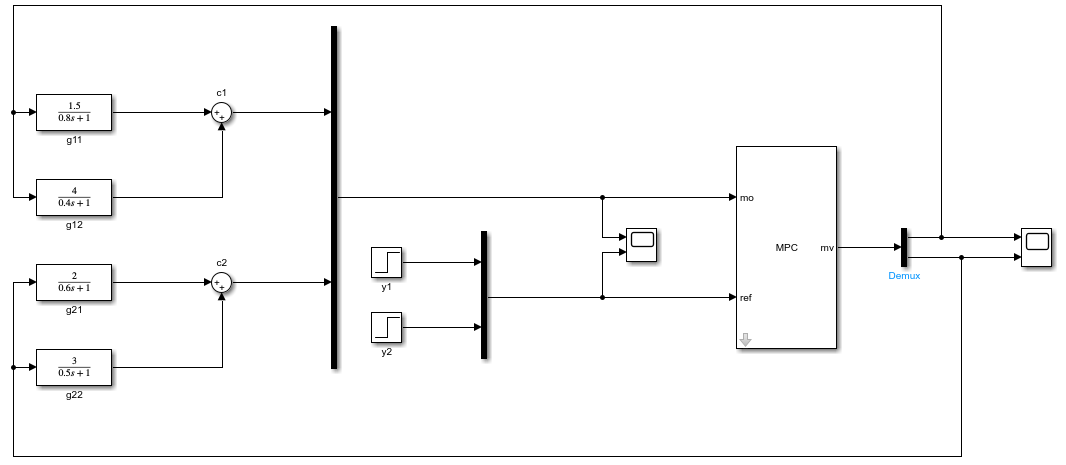
\includegraphics[scale = 0.5]{Q2_sim_layout.png}
		\caption{محیط شبیه‌سازی شده در سیمولینک}
	\end{figure}

در ادامه بلوک کنترلر را با توجه به داده‌های مسئله تنظیم می‌کنیم. پس از تعیین دو ورودی و دو خروجی برای کنترلر، سیگنال‌های مربوطه را انتخاب کرده و به سراغ تنظیم پارامترهای کنترلر می‌رویم.\\
در این مرحله ابتدا قیود مسئله را تعریف می‌کنیم.\\
	\begin{figure}[h!]
	\centering
	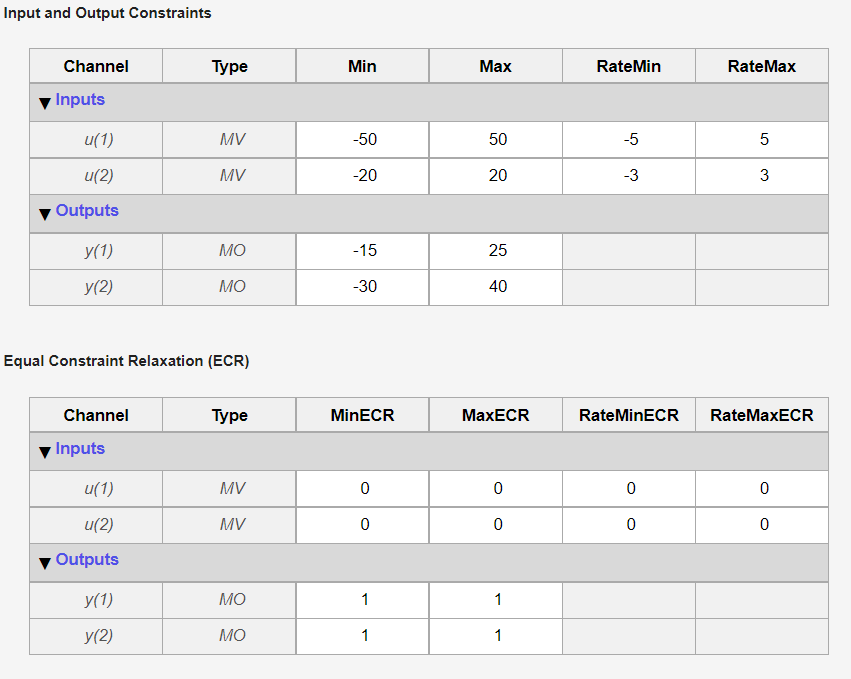
\includegraphics[scale = 0.6]{Q2_sim_constraints.png}
	\caption{صفحه مربوط به قیود در کنترلر}
	\end{figure}

\newpage
سپس وزن‌های داده شده در سوال را در قسمت مربوطه وارد می‌کنیم.\\
	\begin{figure}[h!]
	\centering
	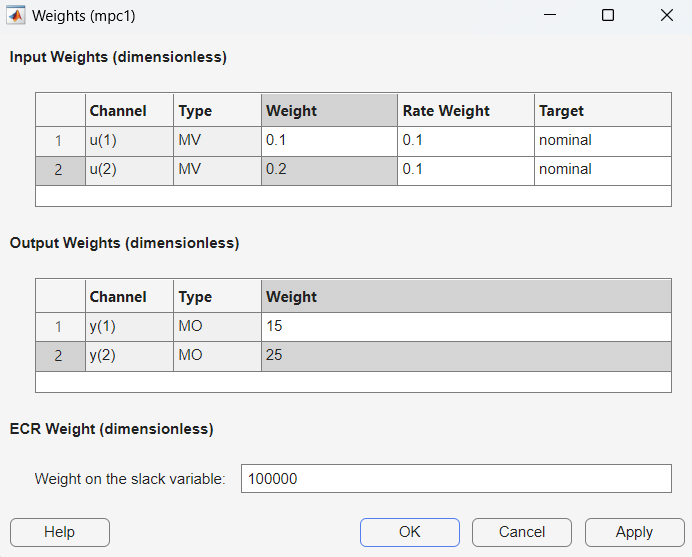
\includegraphics[scale = 0.6]{Q2_sim_weights.png}
	\caption{صفحه مربوط به وزن‌ها در کنترلر}
	\end{figure}

پس از آن، مقادیر مربوط به قیود را انتخاب کرده و عملکرد مدل را بررسی کردیم.\\
	\begin{figure}[h!]
	\centering
	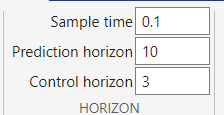
\includegraphics[scale = 1]{Q2_sim_horizon.png}
	\caption{قسمت مربوط به پارامترهای باقیمانده}
	\end{figure}

در ادامه، نتیجه پارامترهای انتخاب شده را با بررسی اسکوپ قرار داده شده مشاهده می‌کنیم.
	\begin{figure}[h!]
	\centering
	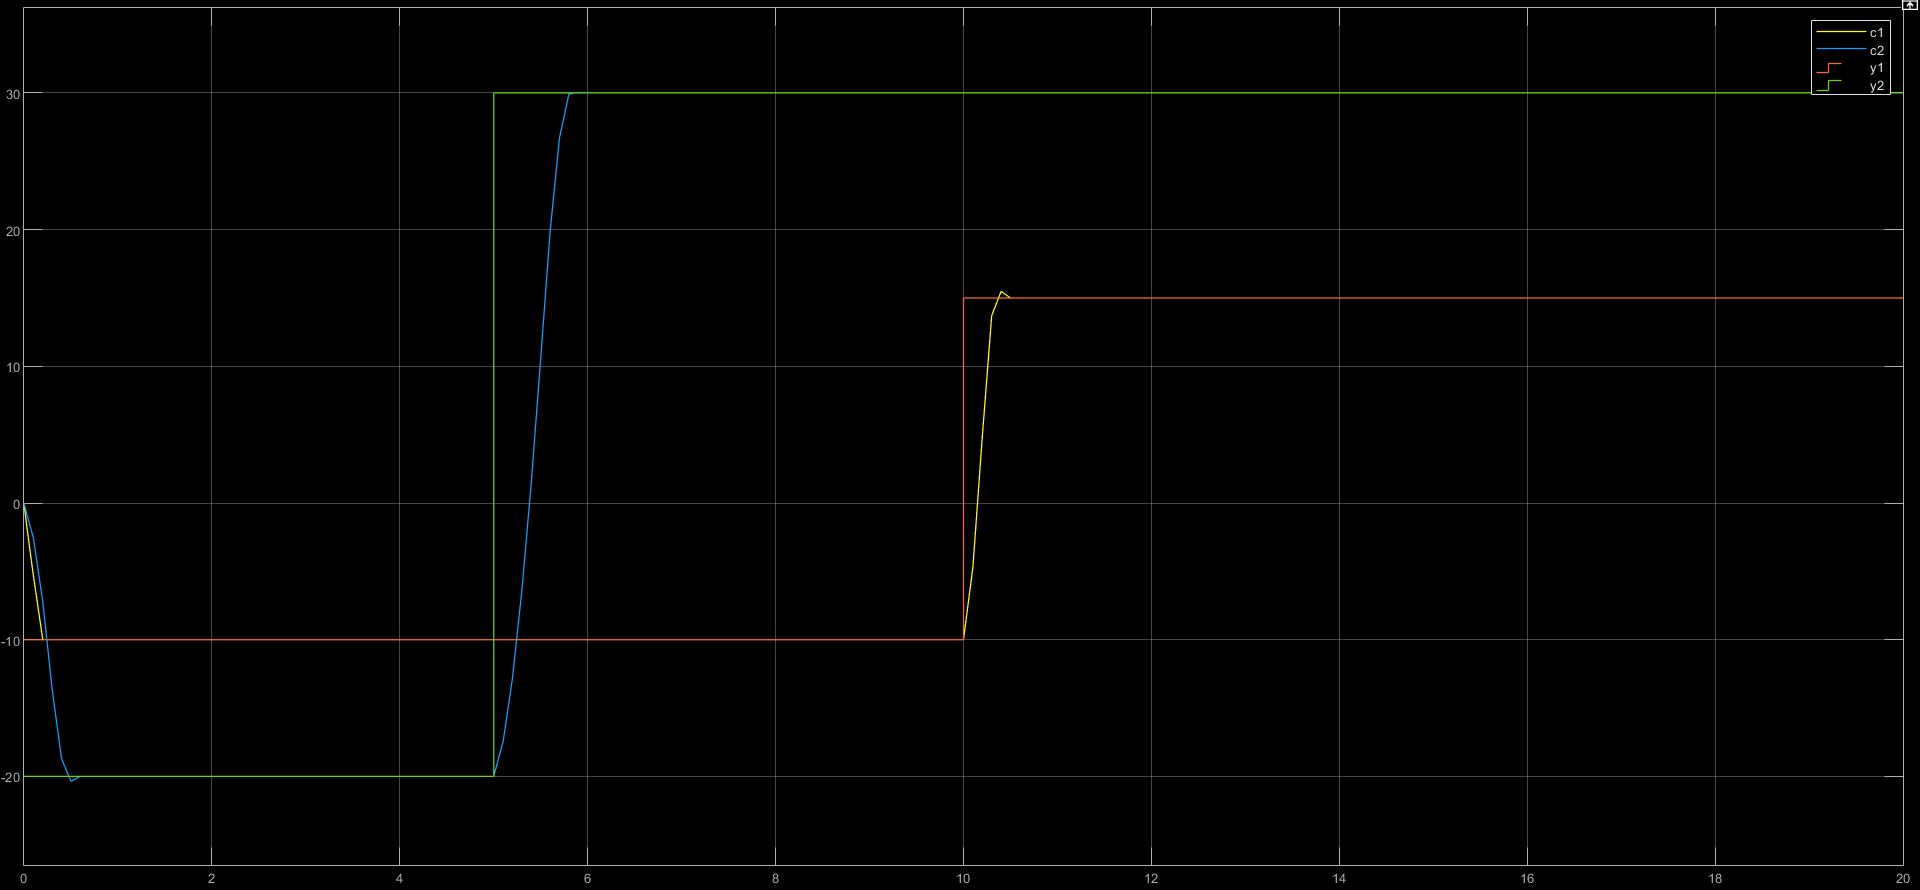
\includegraphics[scale = 0.3]{Q2_sim_result.png}
	\caption{خروجی سیستم کنترل شده}
	\end{figure}

همانطور که از خروجی هم مشخص است، سیستم توانسته با کنترلر طراحی شده به خوبی مقادیر مدنظر را دنبال کرده و با سرعت بالا و فراجهش کم به مقدار نهایی خود برسد.

\subsection{بخش دوم}
در این بخش با دادن مقادیر متفاوت به پنج پارامتر کنترلر و ثابت نگه داشتن سایر مقادیر نسبت به بخش قبل، تاثیر هر یک را بررسی می‌کنیم. پیش از آن یکبار دیگر خروجی سیستم و سیگنال کنترلی را با مقادیر بخش قبل در اینجا قرار می‌دهیم.\\
\begin{figure}[h!]
	\centering
	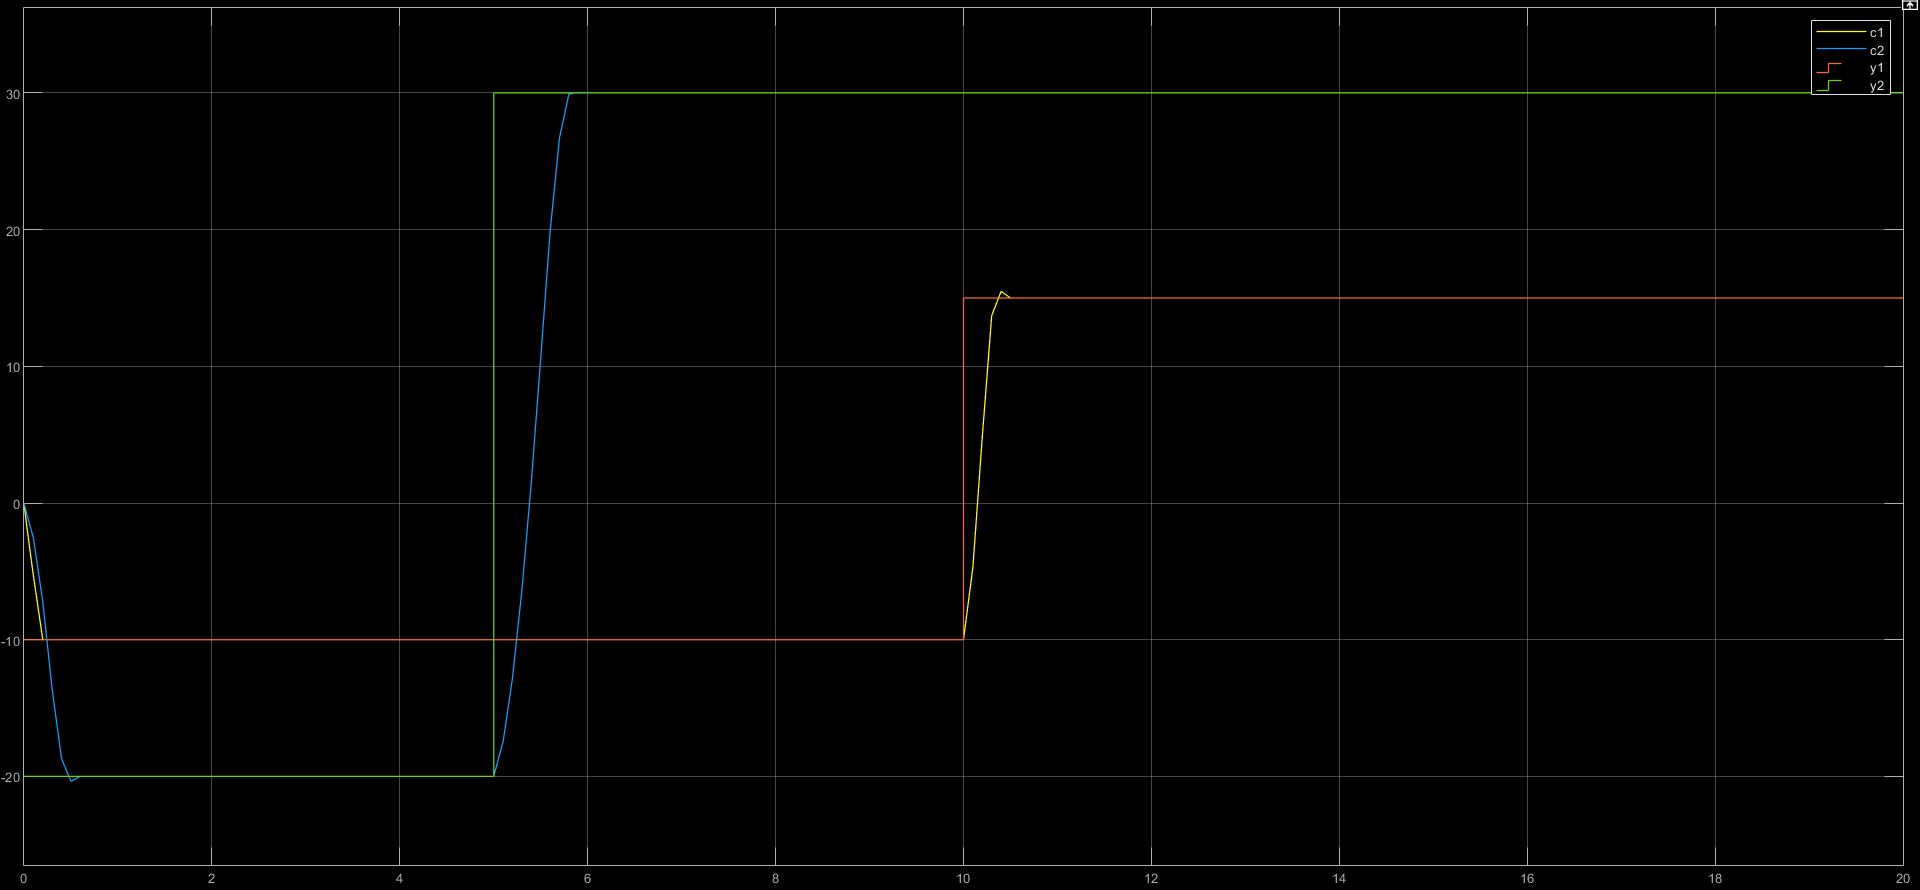
\includegraphics[scale = 0.3]{Q2_sim_result.png}
	\caption{خروجی سیستم کنترل شده}
\end{figure}
\begin{figure}[h!]
	\centering
	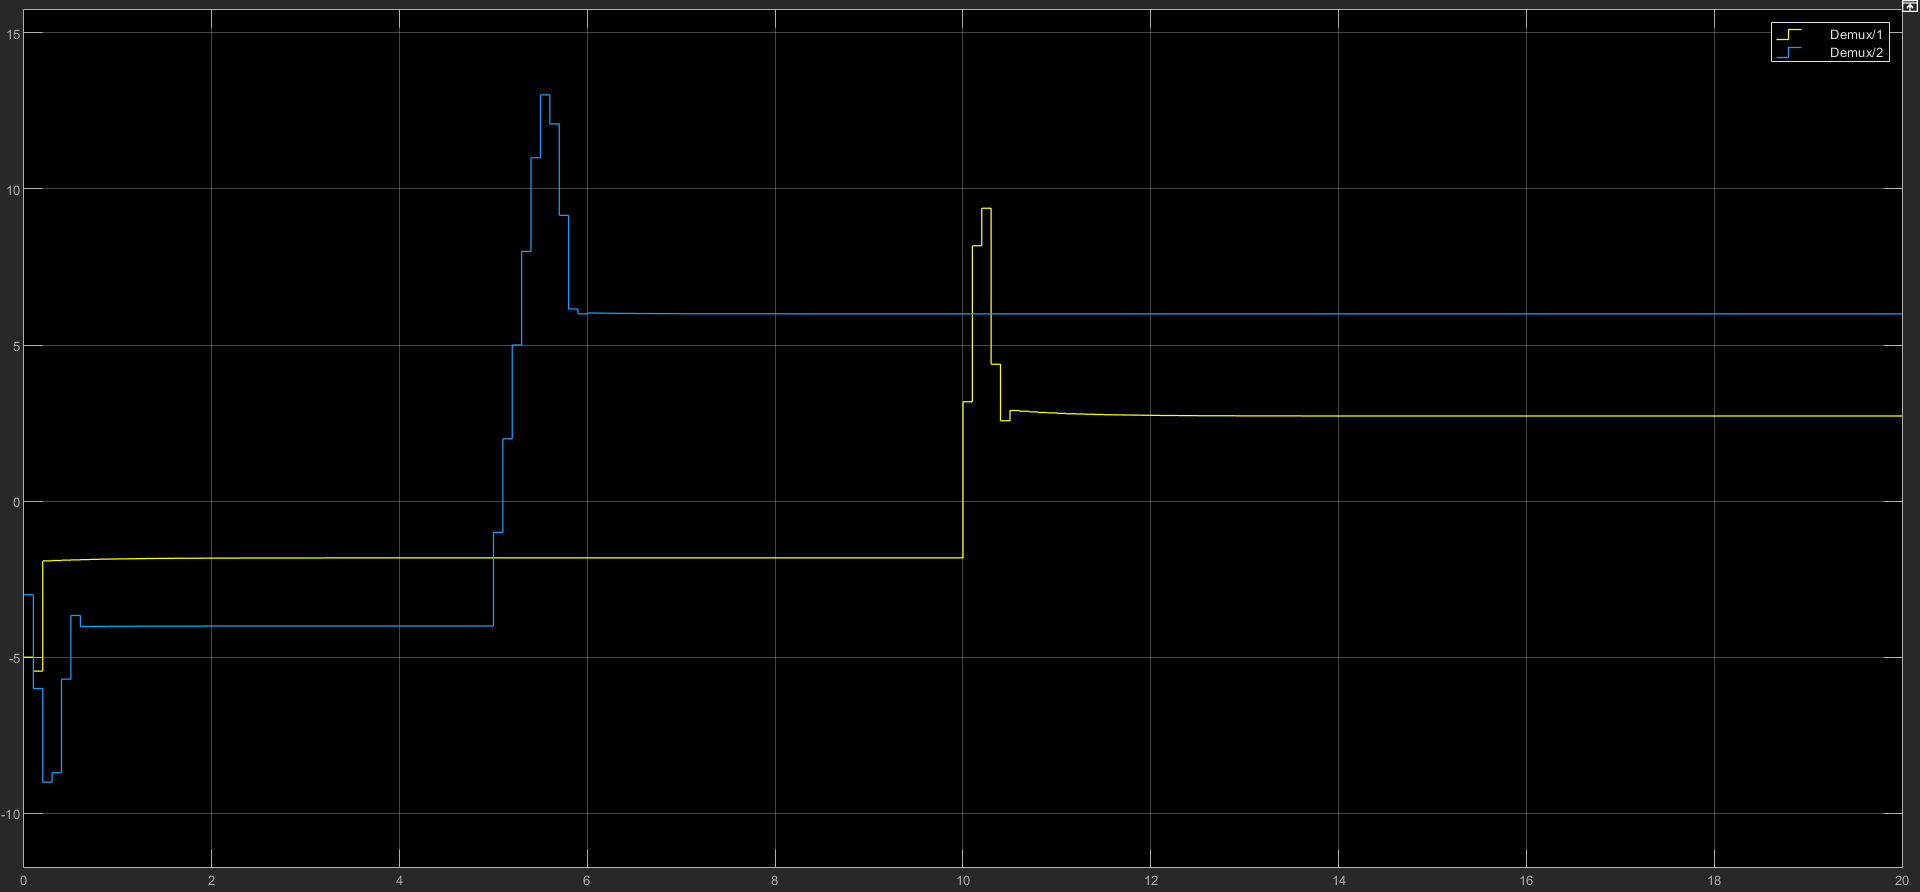
\includegraphics[scale = 0.3]{Q2_sim_control.png}
	\caption{خروجی کنترلر}
\end{figure}

\newpage
\subsubsection{\lr{sample time}}
ابتدا برای 
\lr{sample time = 0.2}
خروجی‌ها را بررسی می‌کنیم.\\
\begin{figure}[h!]
	\centering
	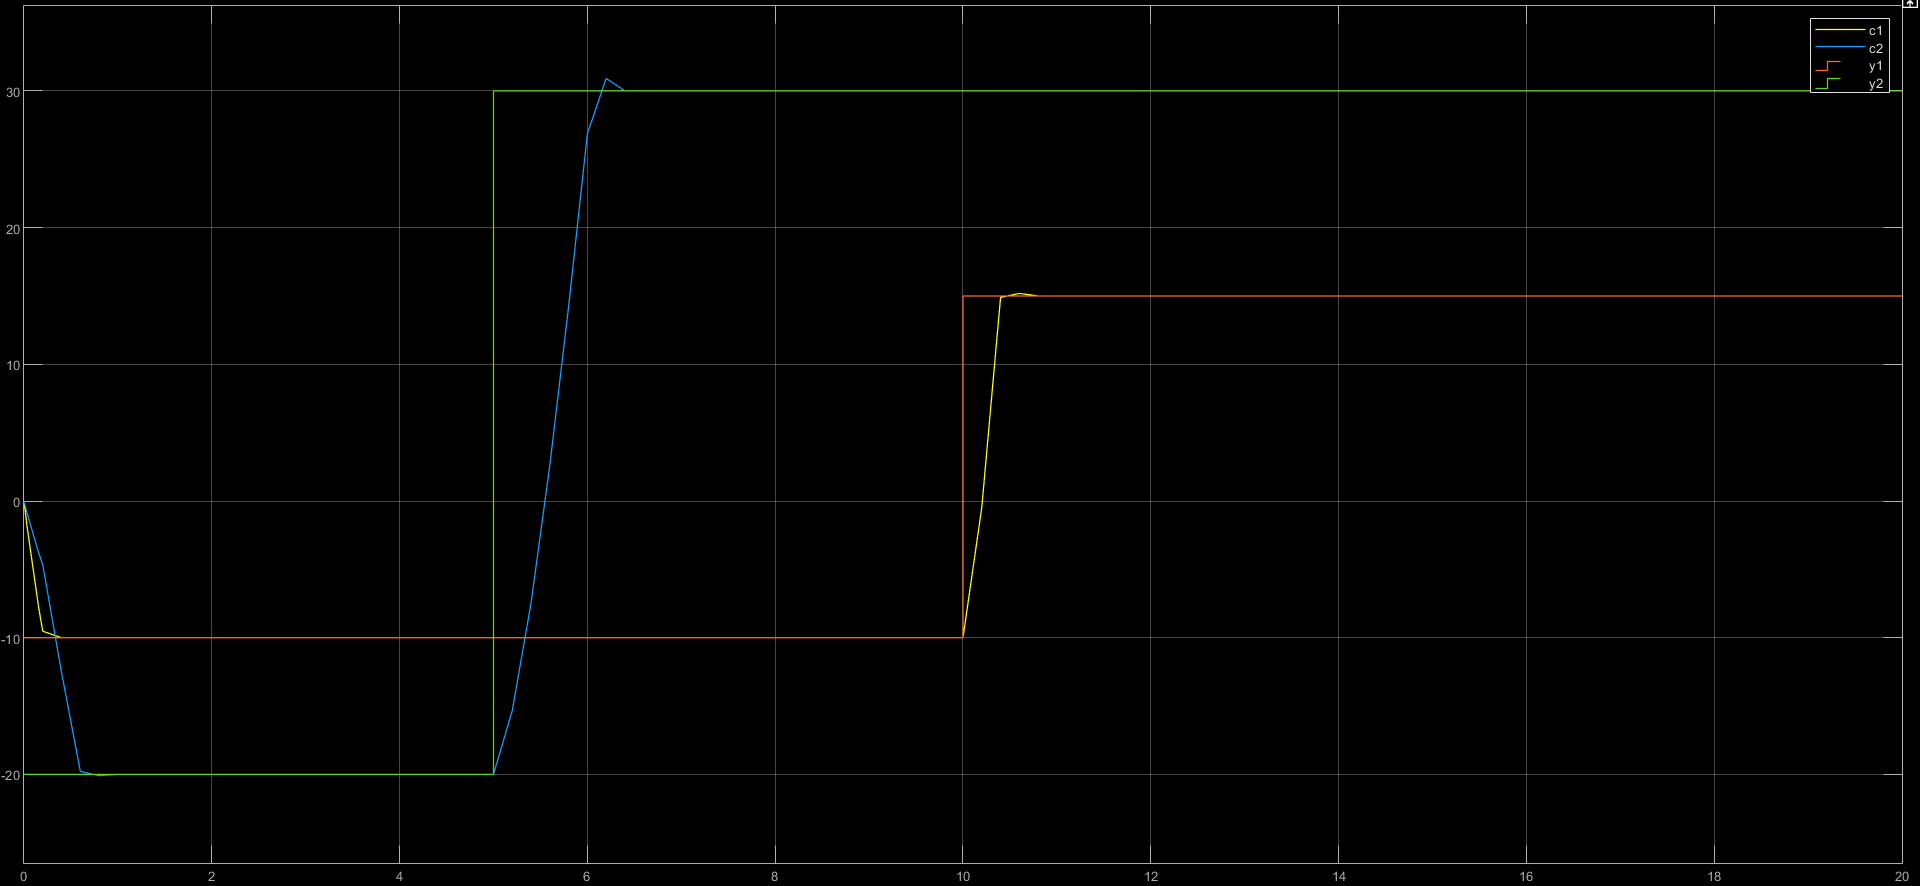
\includegraphics[scale = 0.3]{Q2_sim_result_st02.png}
	\caption{خروجی سیستم کنترل شده با
	\lr{sample time = 0.2}}
\end{figure}
\begin{figure}[h!]
	\centering
	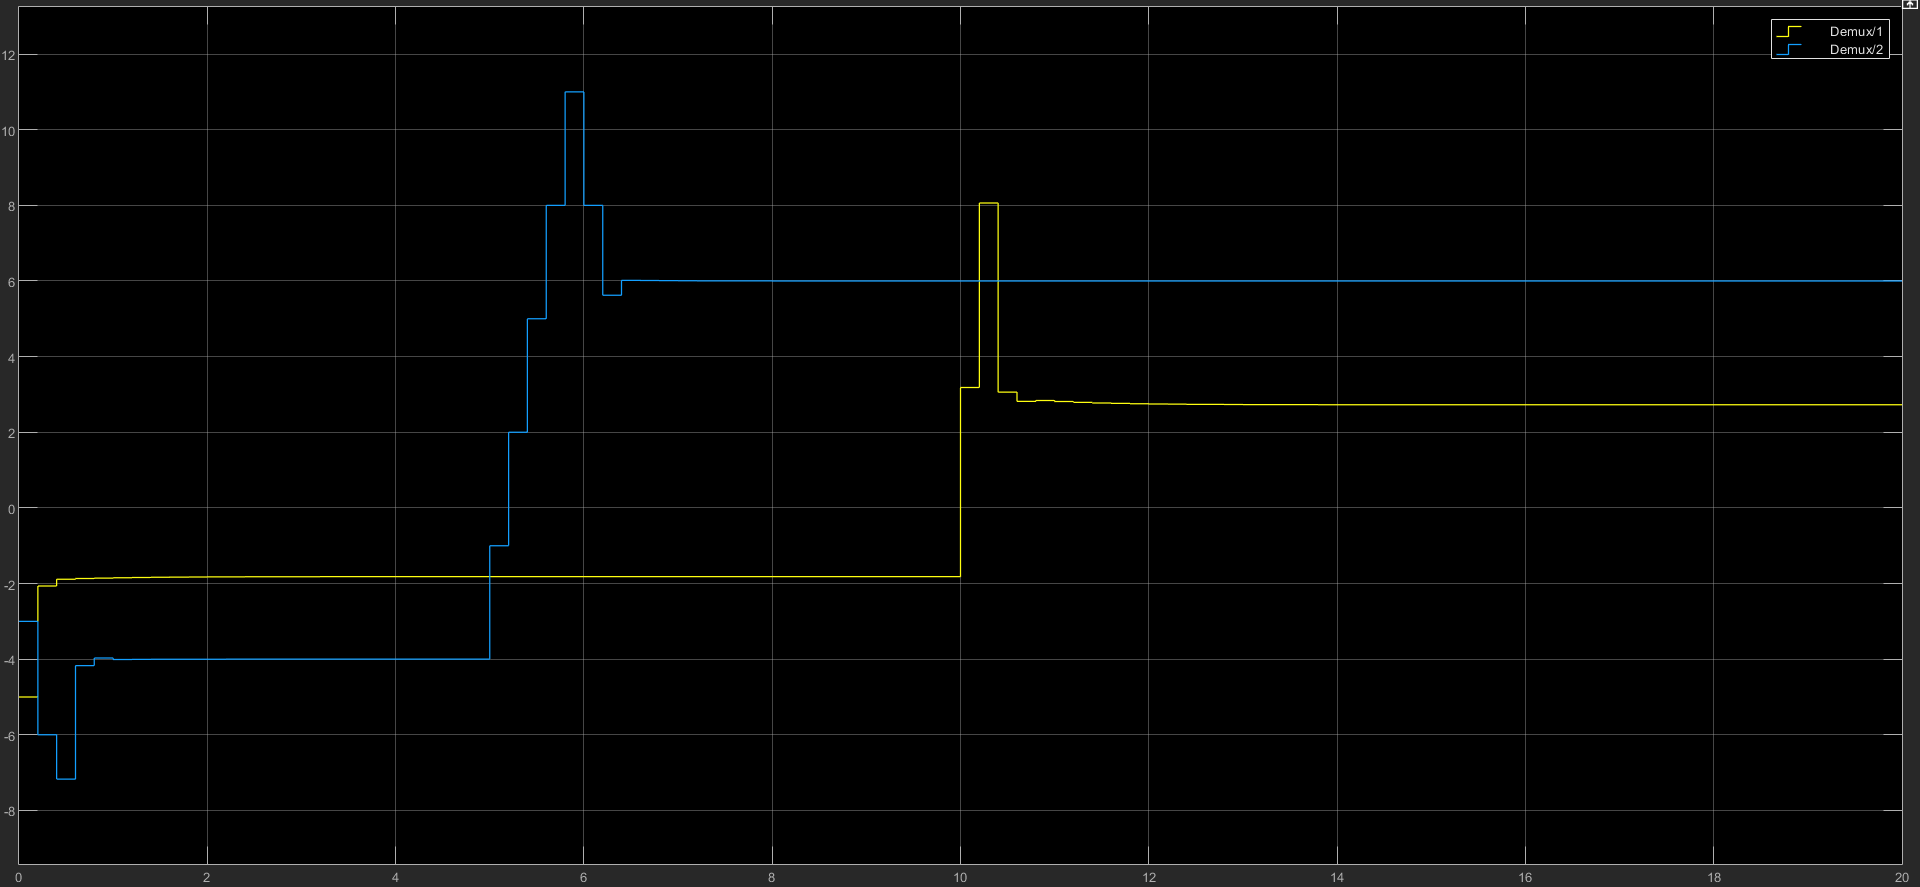
\includegraphics[scale = 0.3]{Q2_sim_control_st02.png}
	\caption{خروجی کنترلر با
	\lr{sample time = 0.2}}
\end{figure}

با افزایش 
\lr{sample time}
خروجی سیستم کندتر و دچار فراجهش بیشتر شده و حداکثر مقدار سیگنال کنترلی (خروجی کنترلر) کاهش یافته است.
\newpage
حال برای 
\lr{sample time = 0.01}
خروجی‌ها را بررسی می‌کنیم.\\
\begin{figure}[h!]
	\centering
	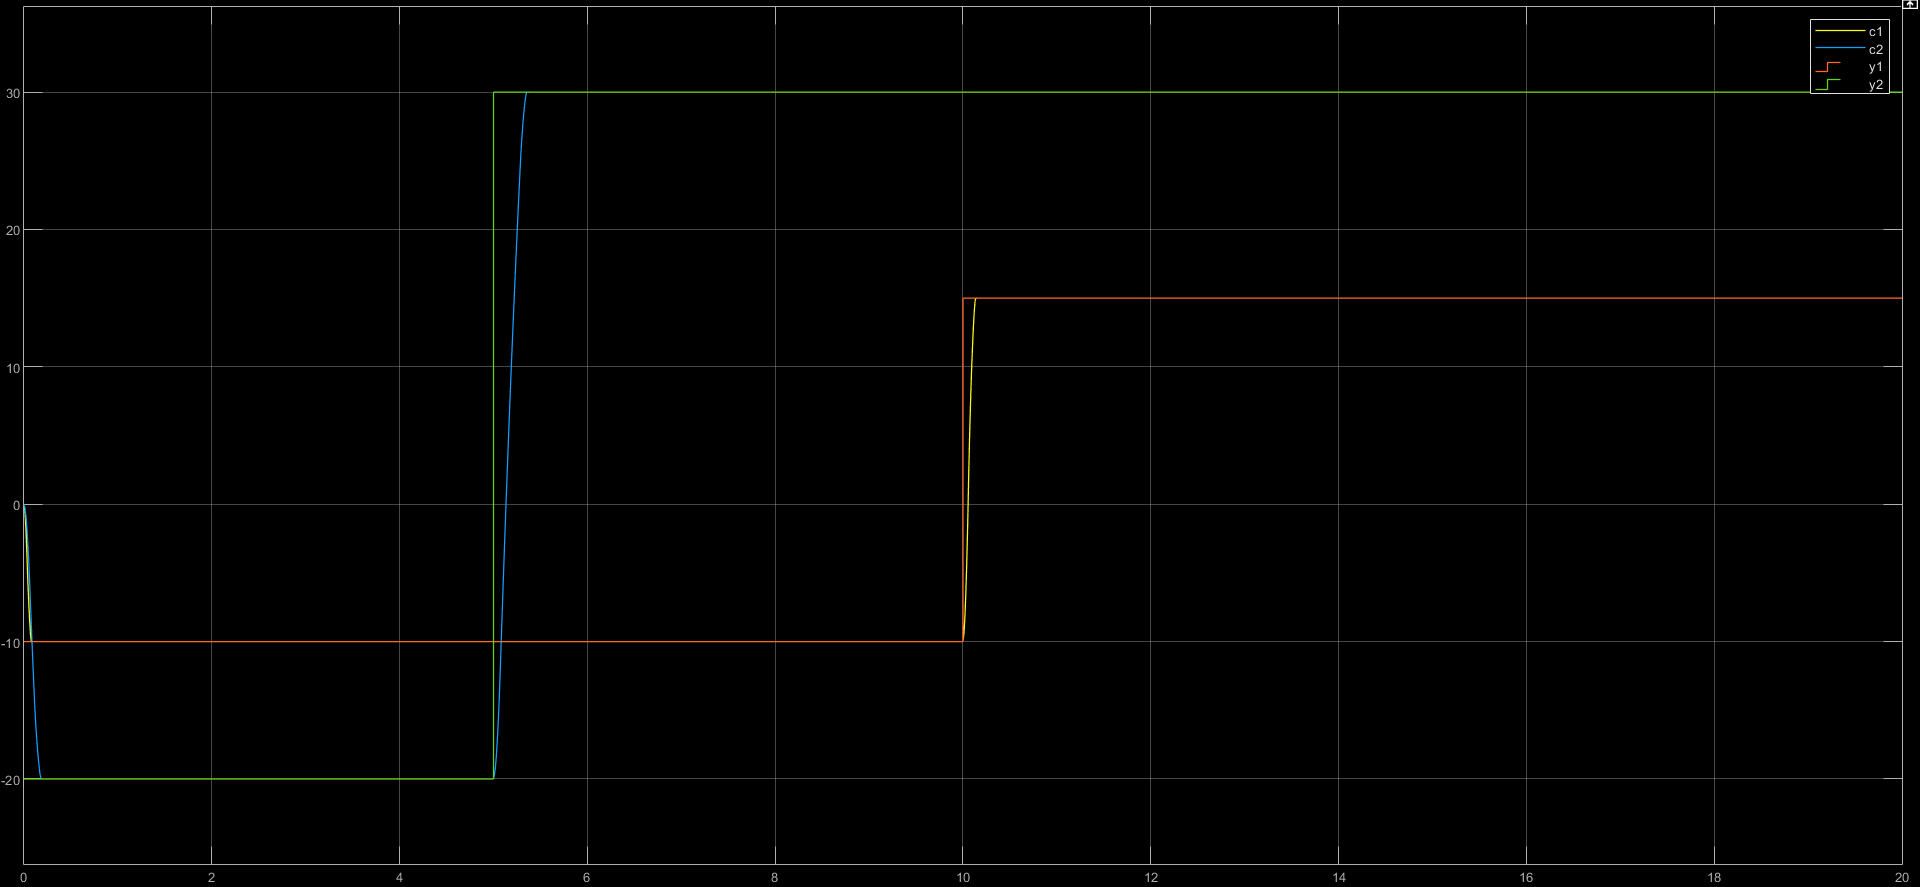
\includegraphics[scale = 0.3]{Q2_sim_result_st001.png}
	\caption{خروجی سیستم کنترل شده با
		\lr{sample time = 0.01}}
\end{figure}
\begin{figure}[h!]
	\centering
	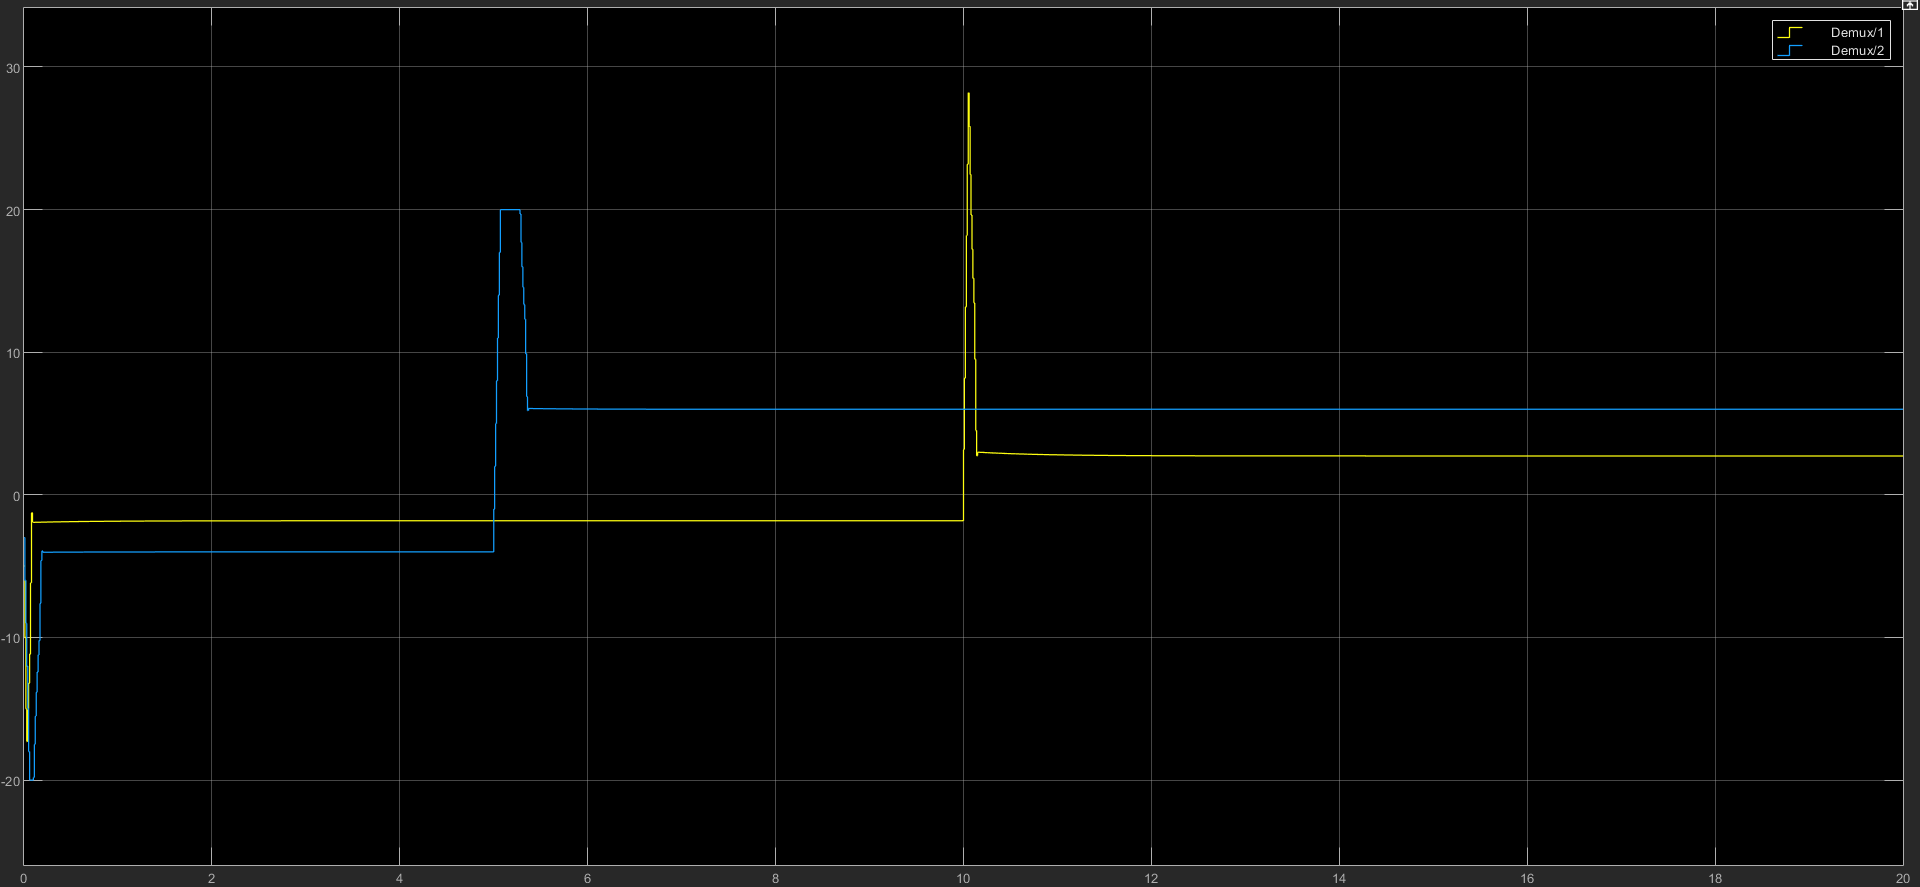
\includegraphics[scale = 0.3]{Q2_sim_control_st001.png}
	\caption{خروجی کنترلر با
		\lr{sample time = 0.01}}
\end{figure}

با کاهش 
\lr{sample time}
خروجی سیستم سریعتر شده و فراجهش آن از بین رفته ولی سیگنال کنترلی (خروجی کنترلر) وارد حالت اشباع شده است که ممکن است مطلوب نباشد.

\newpage
\subsubsection{\lr{Prediction horizon}}
ابتدا برای 
\lr{Prediction horizon = 20}
خروجی‌ها را بررسی می‌کنیم.\\
\begin{figure}[h!]
	\centering
	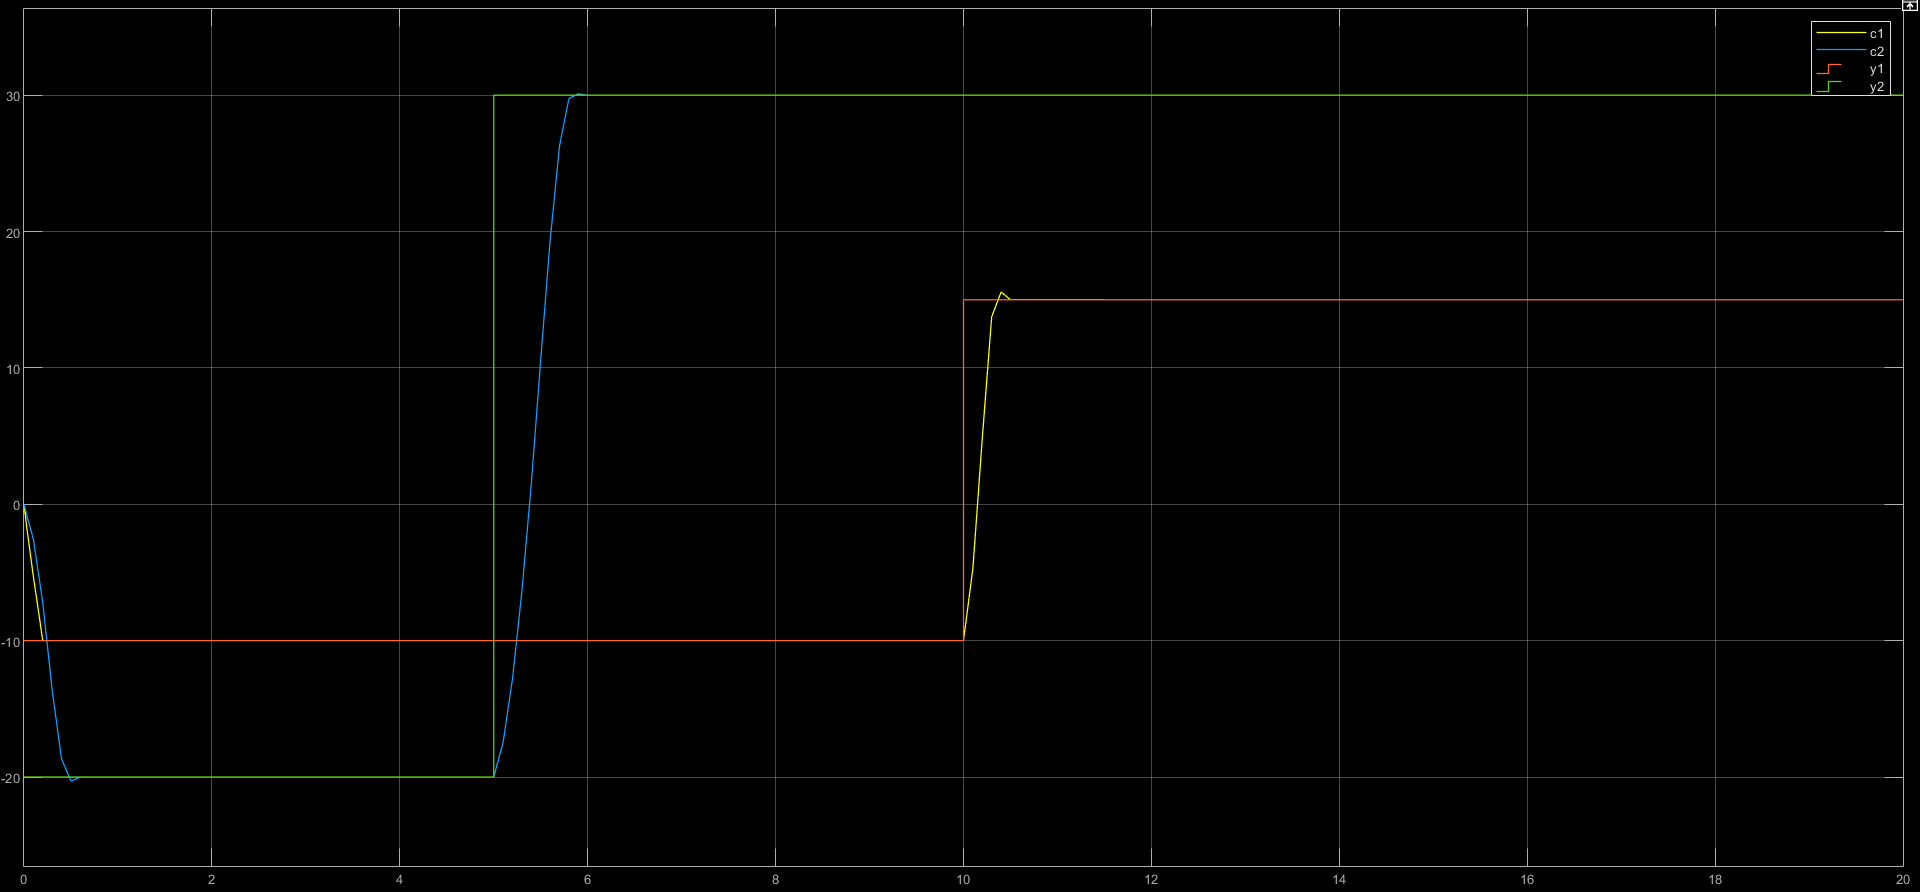
\includegraphics[scale = 0.3]{Q2_sim_result_ph20.png}
	\caption{خروجی سیستم کنترل شده با
		\lr{Prediction horizon = 20}}
\end{figure}
\begin{figure}[h!]
	\centering
	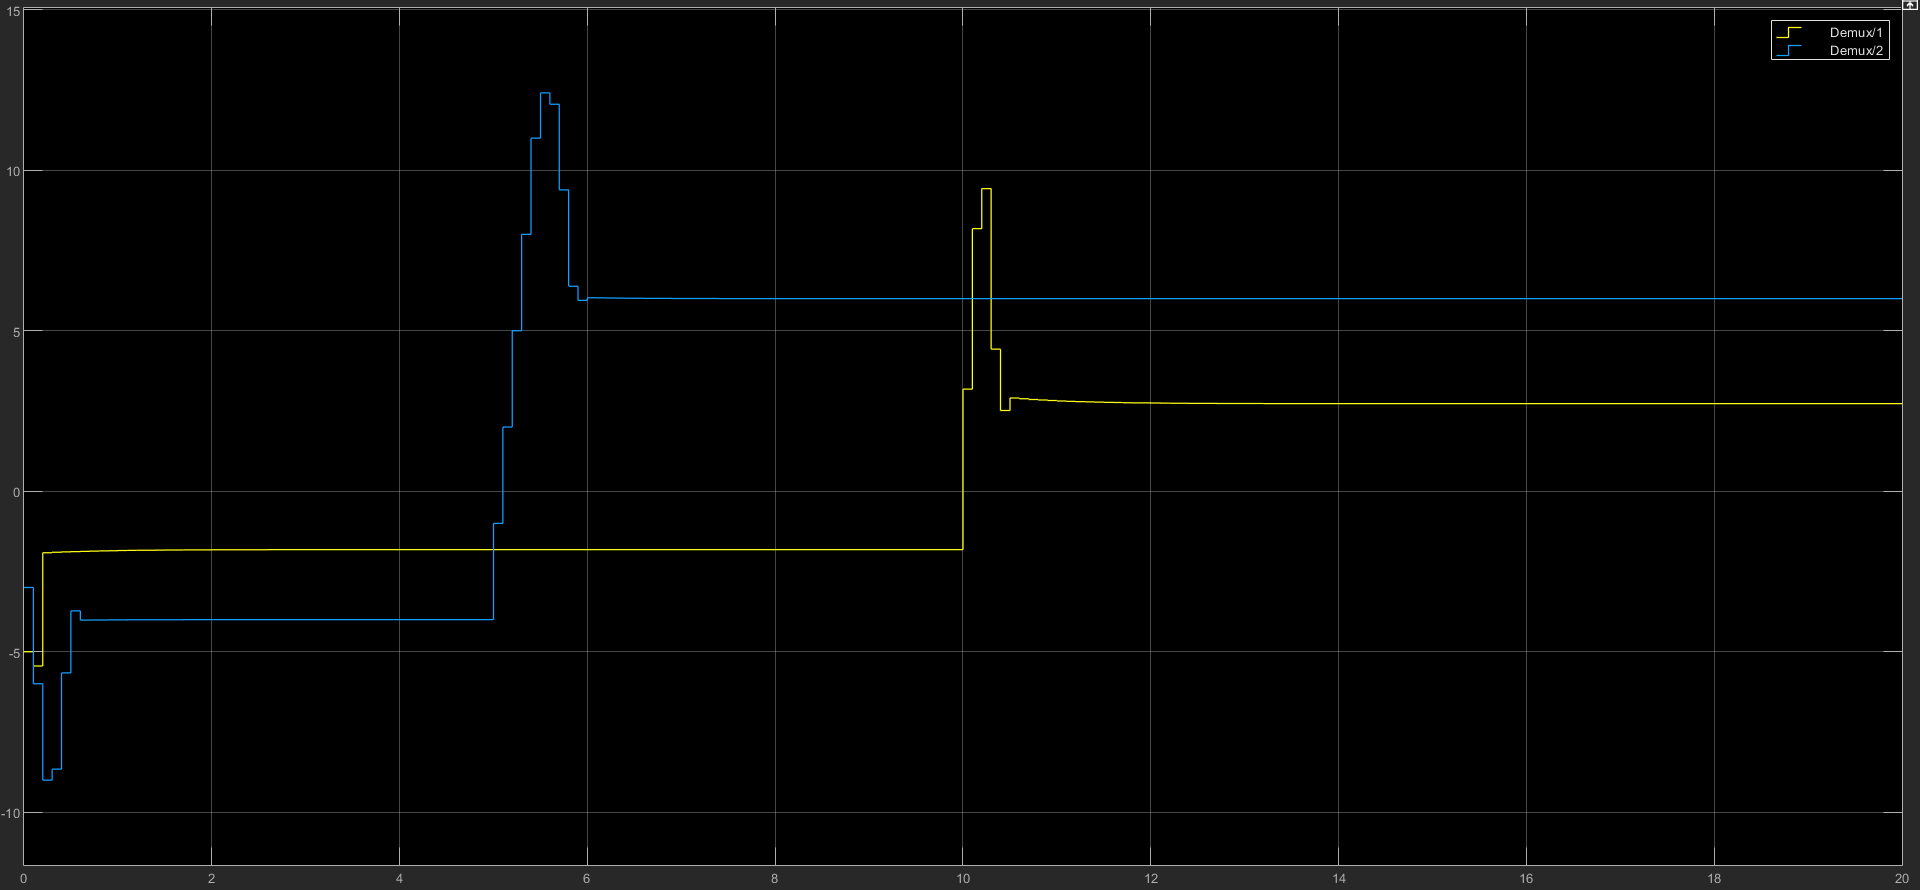
\includegraphics[scale = 0.3]{Q2_sim_control_ph20.png}
	\caption{خروجی کنترلر با
		\lr{Prediction horizon = 20}}
\end{figure}

با افزایش 
\lr{Prediction horizon}
تفییر واضحی در سیستم اتفاق نیفتاده است.
\newpage
حال برای 
\lr{Prediction horizon = 5}
خروجی‌ها را بررسی می‌کنیم.\\
\begin{figure}[h!]
	\centering
	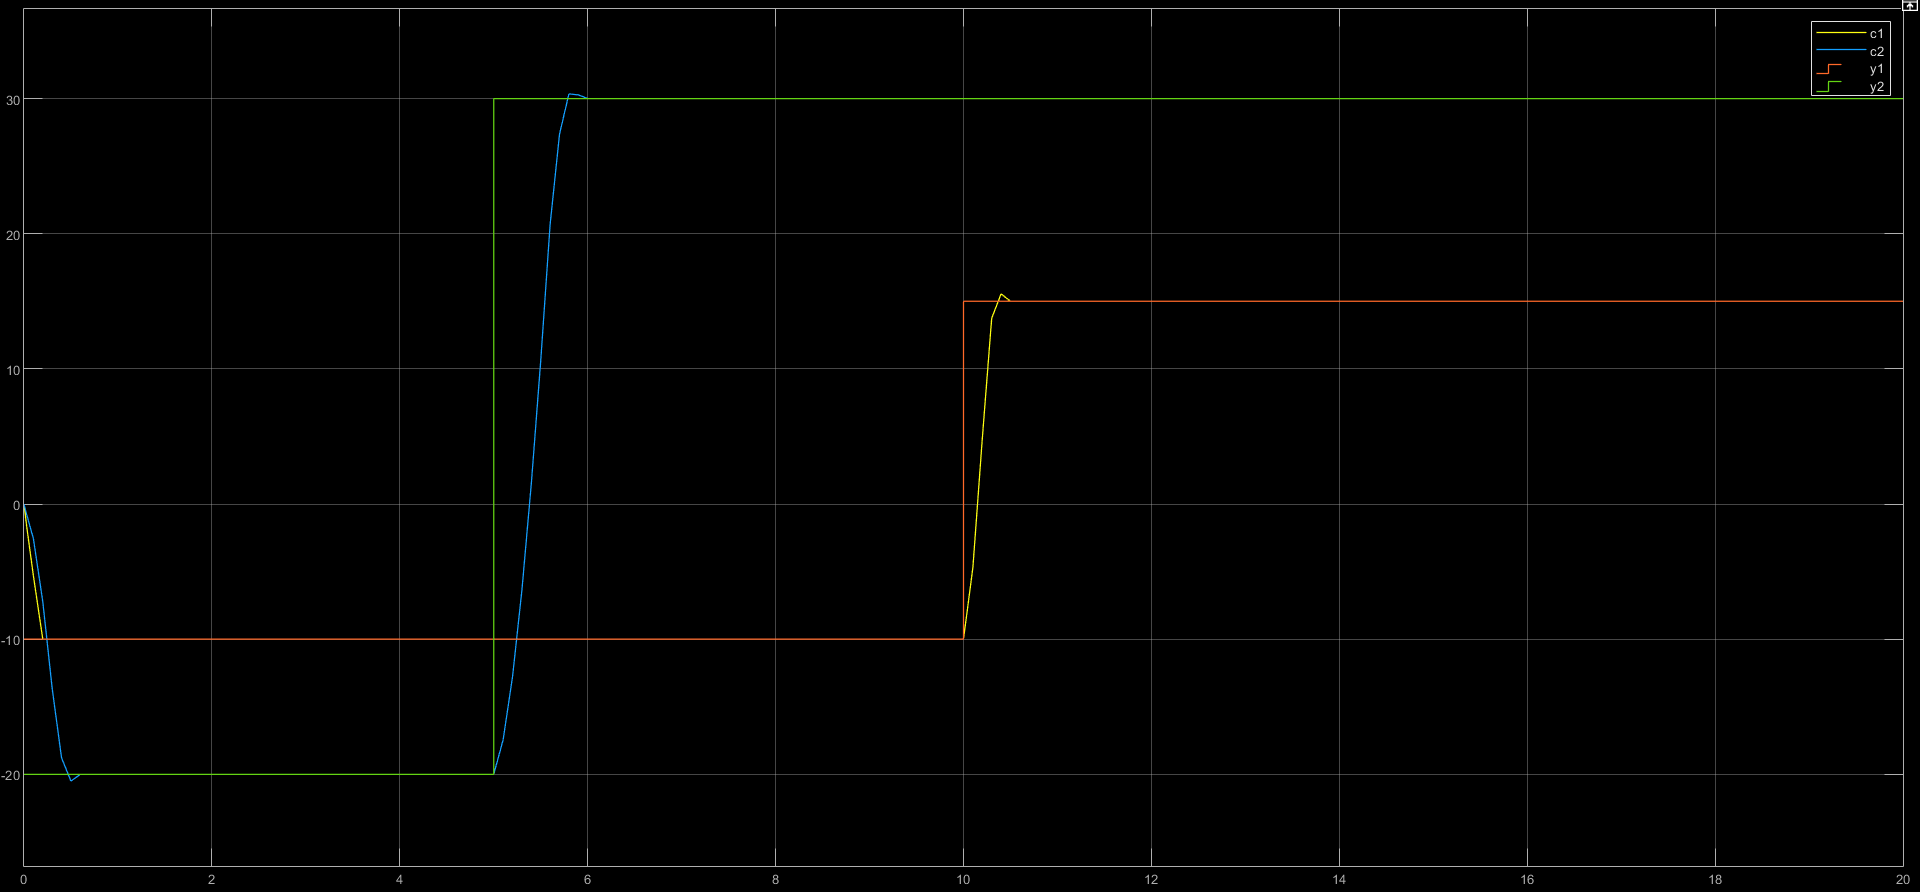
\includegraphics[scale = 0.3]{Q2_sim_result_ph5.png}
	\caption{خروجی سیستم کنترل شده با
		\lr{Prediction horizon = 5}}
\end{figure}
\begin{figure}[h!]
	\centering
	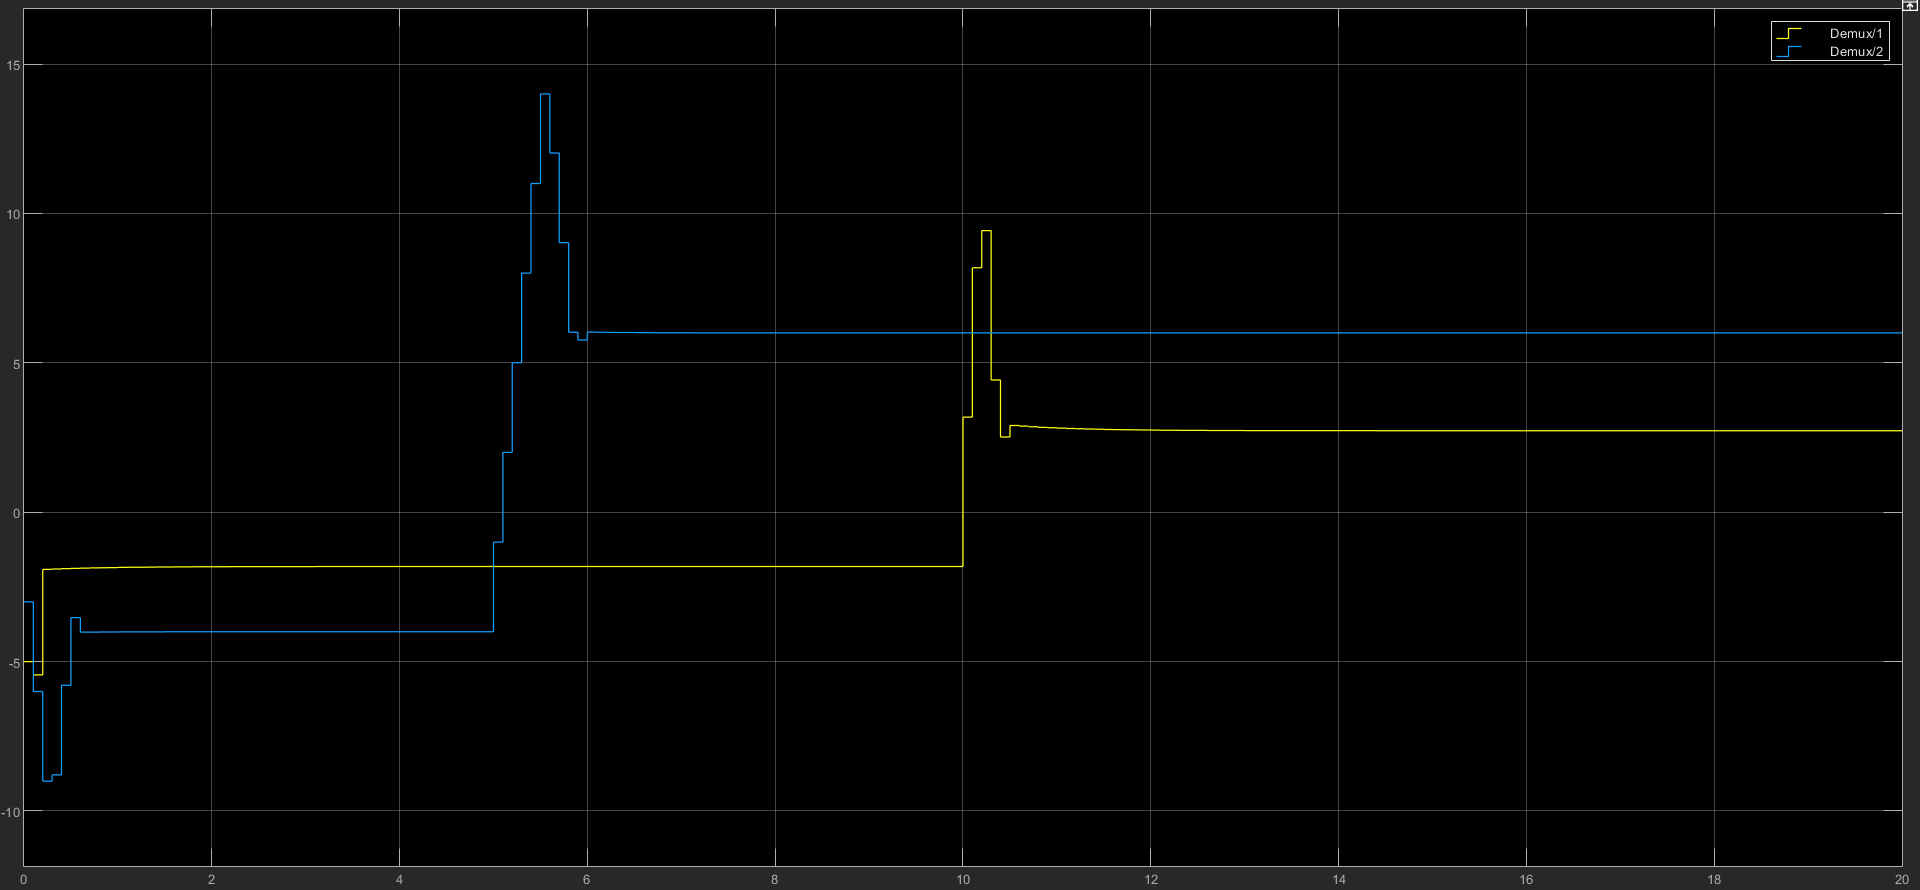
\includegraphics[scale = 0.3]{Q2_sim_control_ph5.png}
	\caption{خروجی کنترلر با
		\lr{Prediction horizon = 5}}
\end{figure}

با کاهش 
\lr{Prediction horizon}
خروجی سیستم، فراجهش آن و سیگنال کنترلی (خروجی کنترلر) همگی اندکی سریعتر شده‌اند.

\newpage
\subsubsection{\lr{Control horizon}}
ابتدا برای 
\lr{Control horizon = 5}
خروجی‌ها را بررسی می‌کنیم.\\
\begin{figure}[h!]
	\centering
	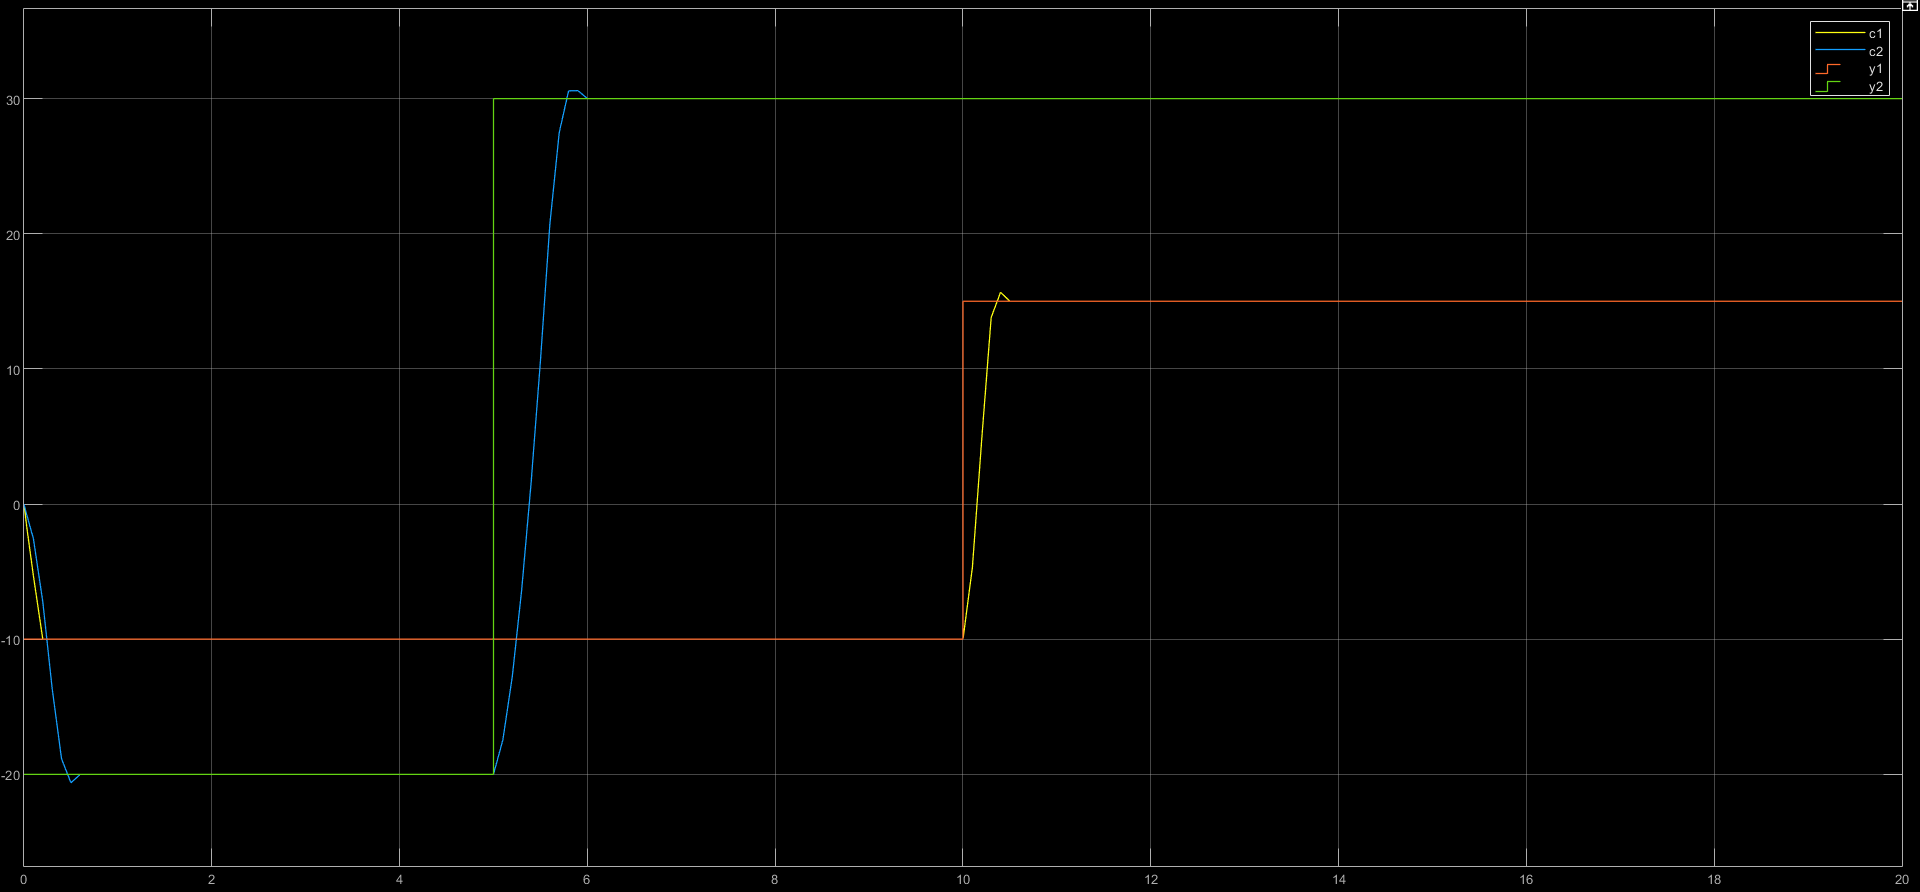
\includegraphics[scale = 0.3]{Q2_sim_result_ch5.png}
	\caption{خروجی سیستم کنترل شده با
		\lr{Control horizon = 5}}
\end{figure}
\begin{figure}[h!]
	\centering
	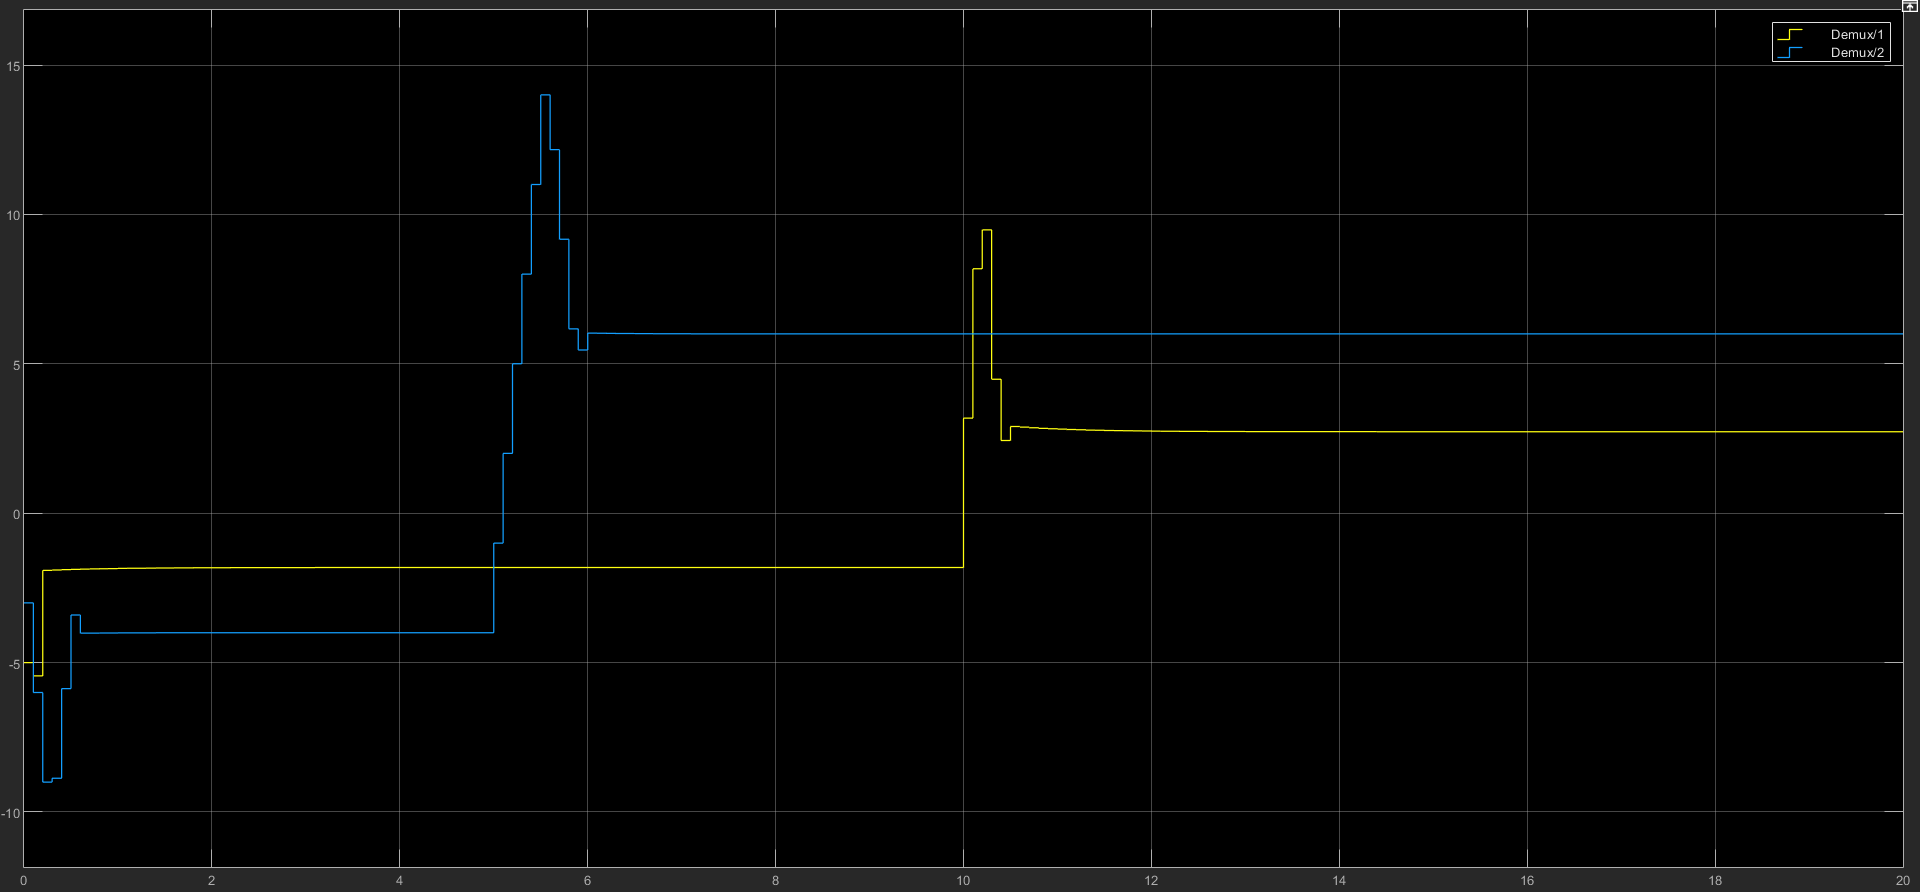
\includegraphics[scale = 0.3]{Q2_sim_control_ch5.png}
	\caption{خروجی کنترلر با
		\lr{Control horizon = 5}}
\end{figure}

با افزایش 
\lr{Control horizon}
خروجی سیستم، فراجهش آن و سیگنال کنترلی (خروجی کنترلر) همگی اندکی سریعتر شده‌اند.
\newpage
حال برای 
\lr{Control horizon = 1}
خروجی‌ها را بررسی می‌کنیم.\\
\begin{figure}[h!]
	\centering
	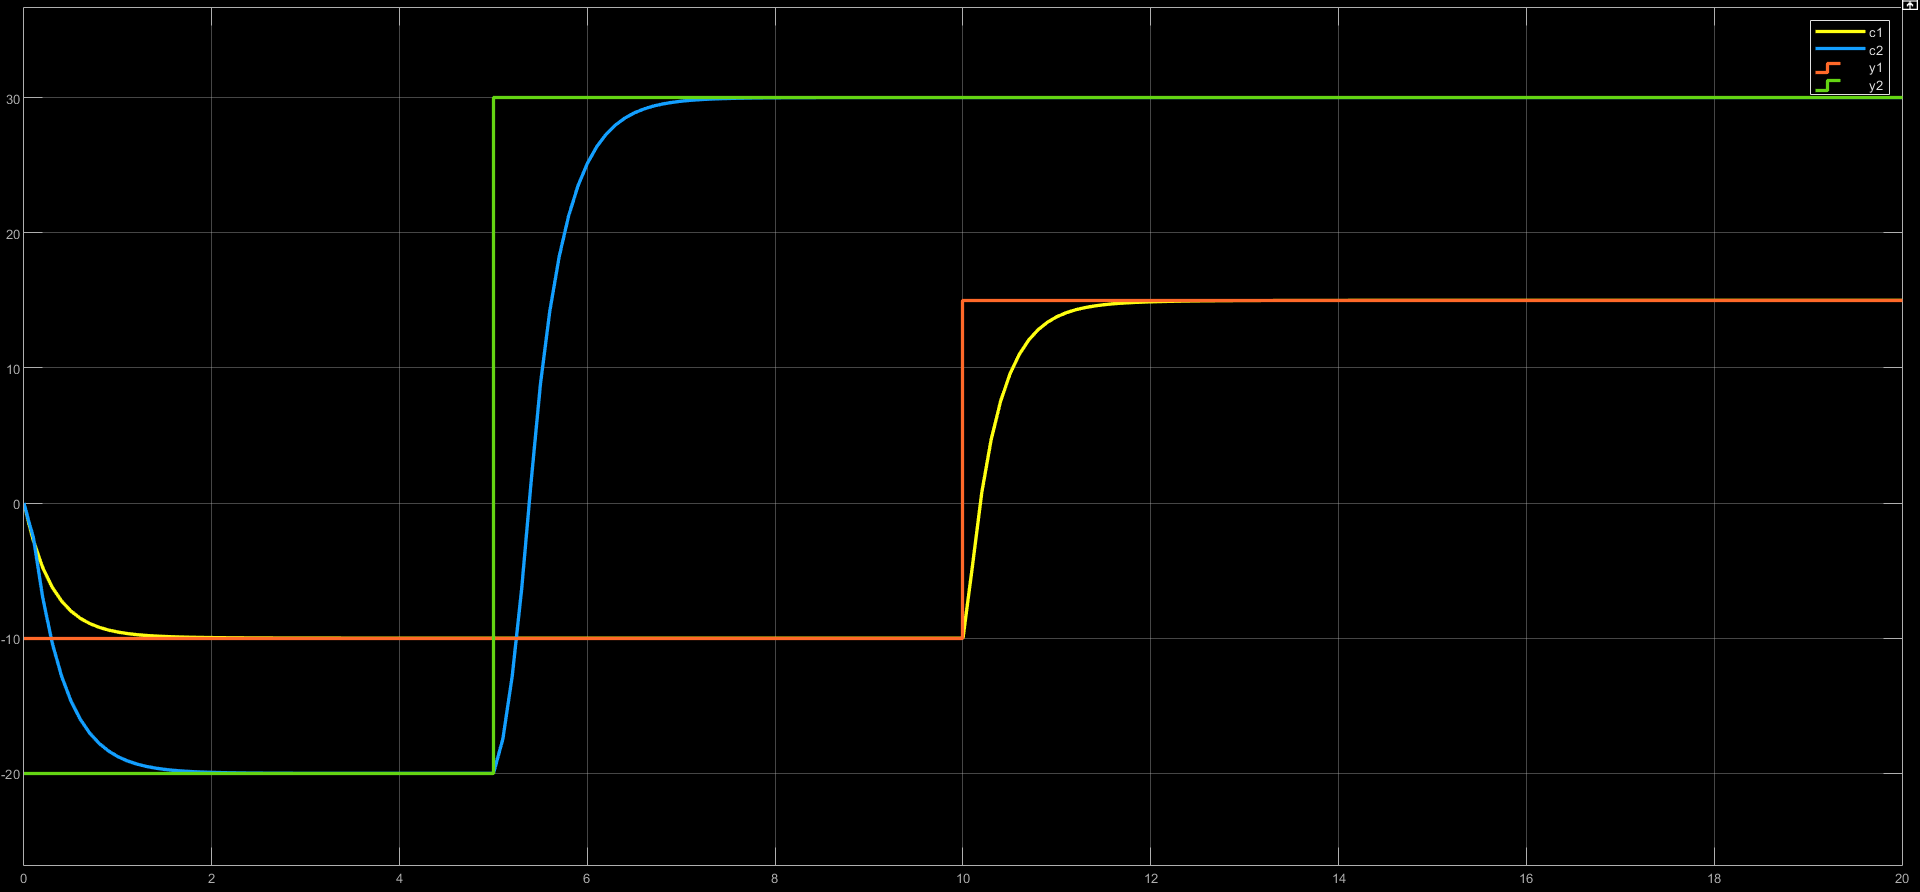
\includegraphics[scale = 0.3]{Q2_sim_result_ch1.png}
	\caption{خروجی سیستم کنترل شده با
		\lr{Control horizon = 1}}
\end{figure}
\begin{figure}[h!]
	\centering
	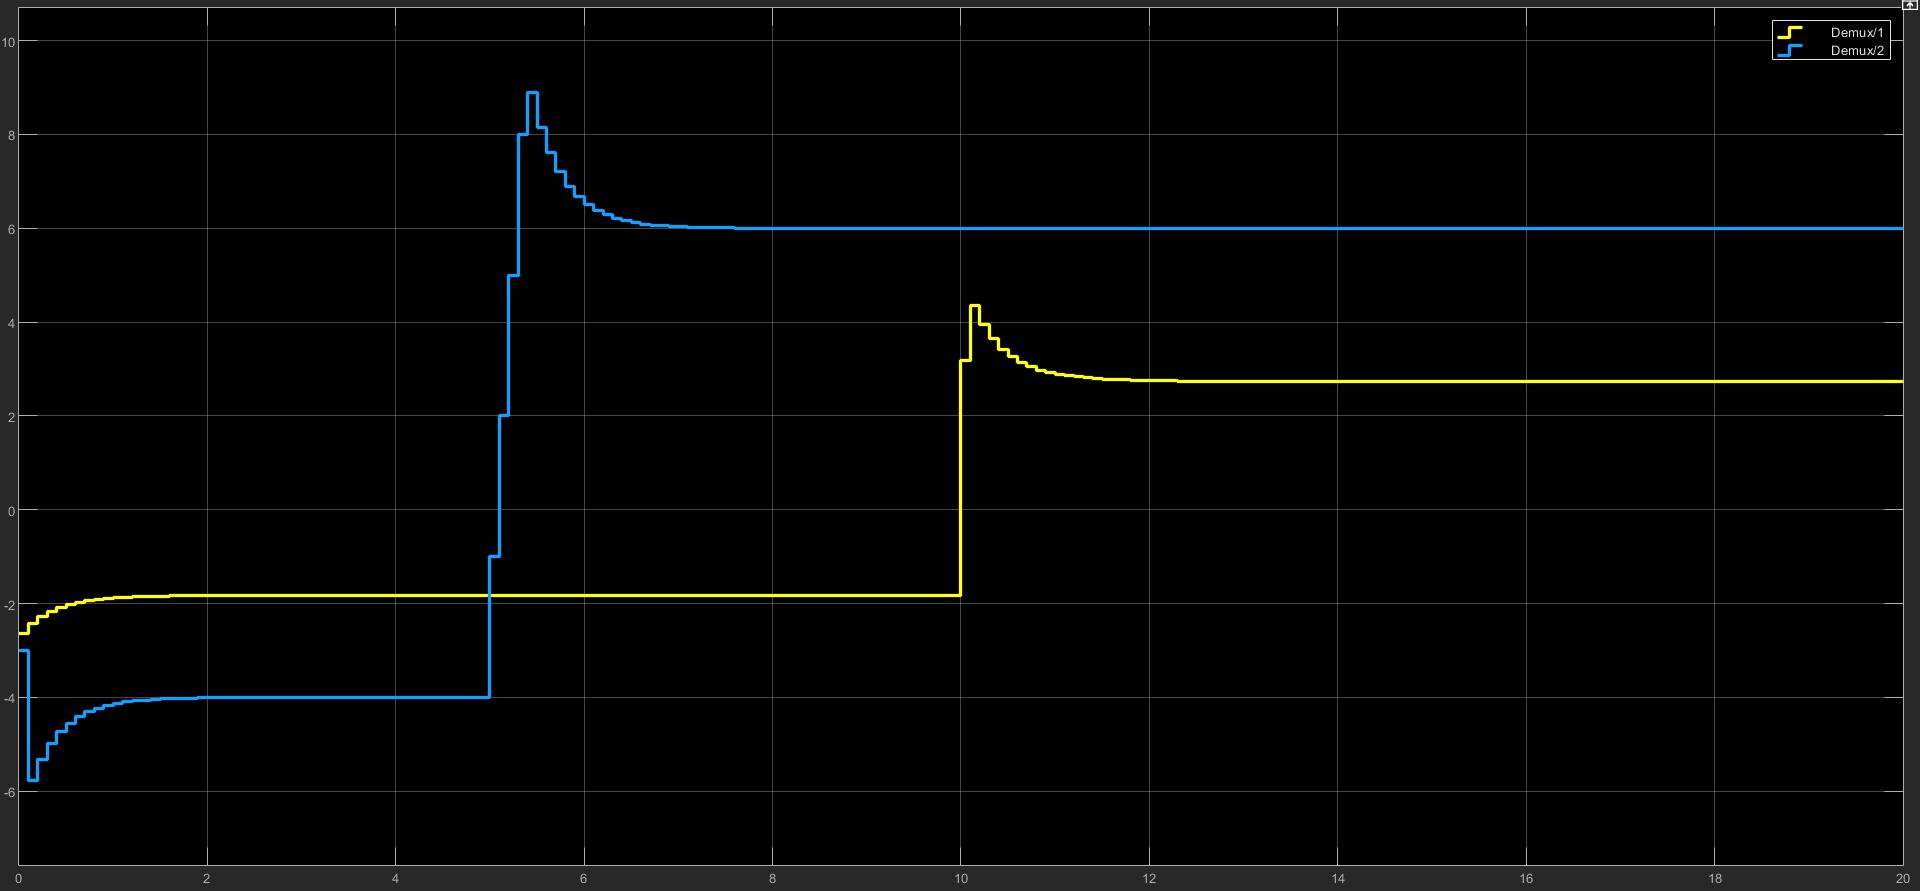
\includegraphics[scale = 0.3]{Q2_sim_control_ch1.png}
	\caption{خروجی کنترلر با
		\lr{Control horizon = 1}}
\end{figure}

با کاهش 
\lr{Control horizon}
خروجی سیستم، فراجهش آن و سیگنال کنترلی (خروجی کنترلر) همگی کاهش محسوس داشته و کند شده‌اند.

\newpage
\subsubsection{\lr{Constraints}}
تغییر در مقادیر حداکثر و حداقل ورودی و سیگنال کنترلی تاثیر خود را فقط در وضعیت اشباع سیستم نمایش می‌دهند. از این جهت صرفا تغییرات نرخ تغییر را بررسی خواهیم کرد.\\
ابتدا برای نرخ تغییر با بازه کوچکتر خروجی‌ها را بررسی می‌کنیم.\\
\[
-3 W/min \leq \dot{u}_1 \leq 3 W/min
\]
\[
-1 W/min \leq \dot{u}_2 \leq 1 W/min
\]
\begin{figure}[h!]
	\centering
	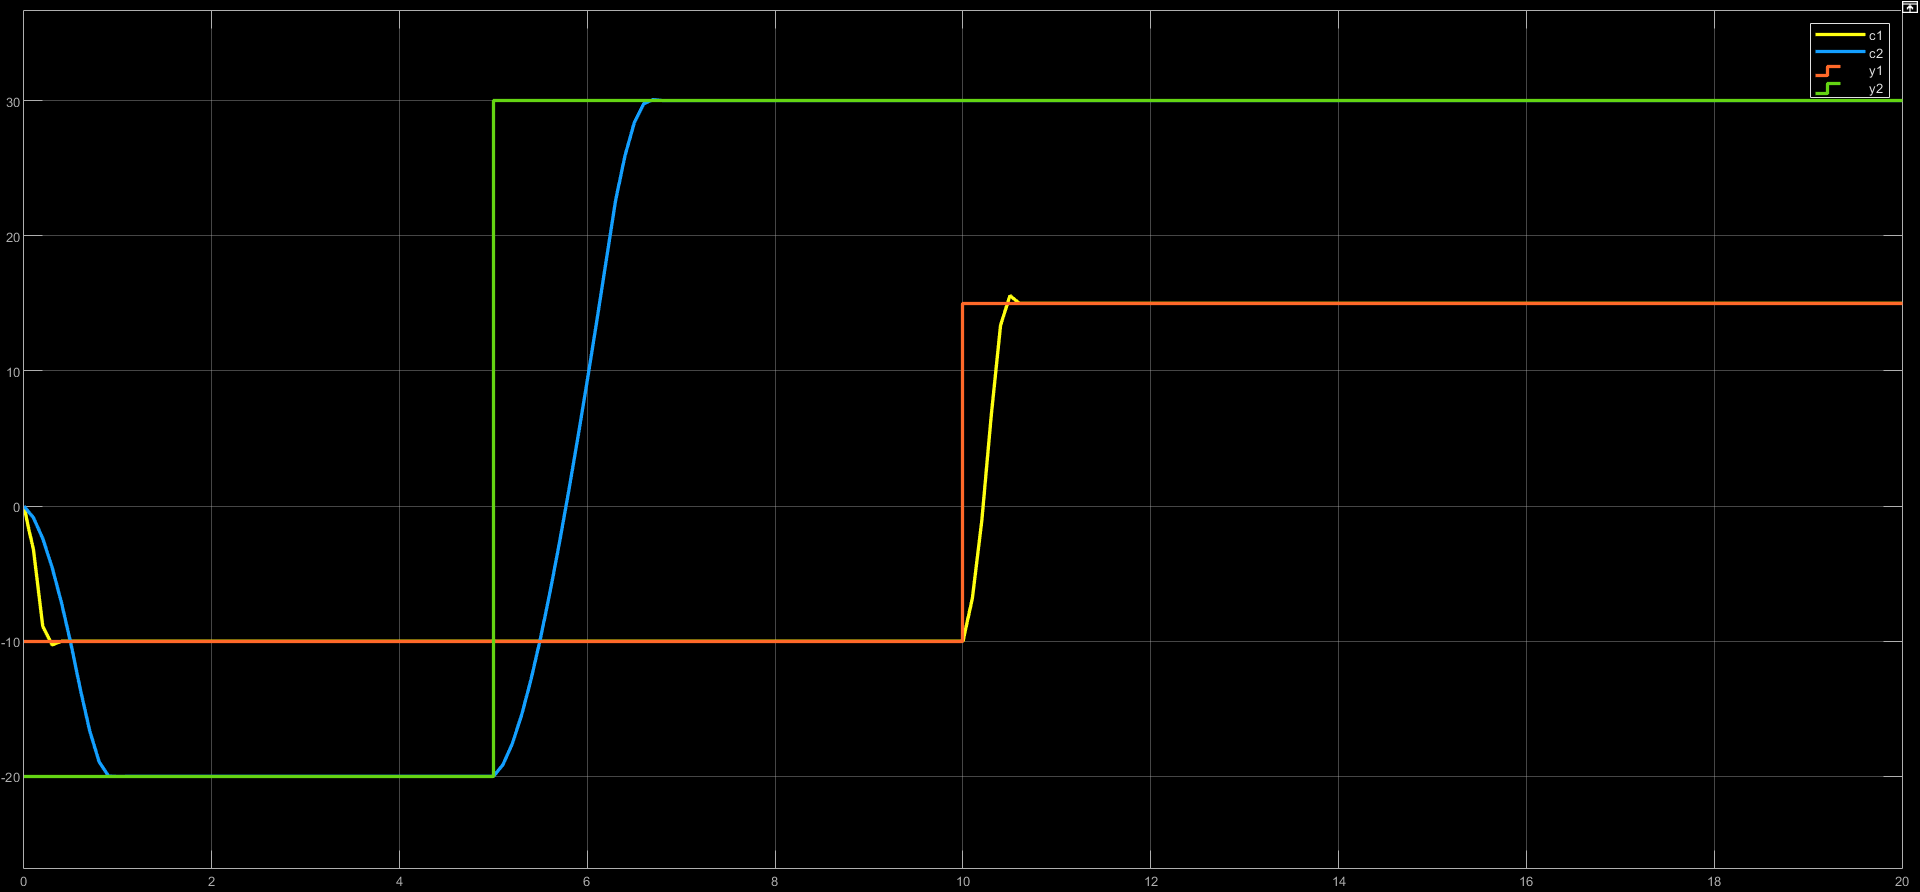
\includegraphics[scale = 0.3]{Q2_sim_result_consmall.png}
	\caption{خروجی سیستم کنترل شده با
		نرخ تغییر با بازه کوچکتر}
\end{figure}
\begin{figure}[h!]
	\centering
	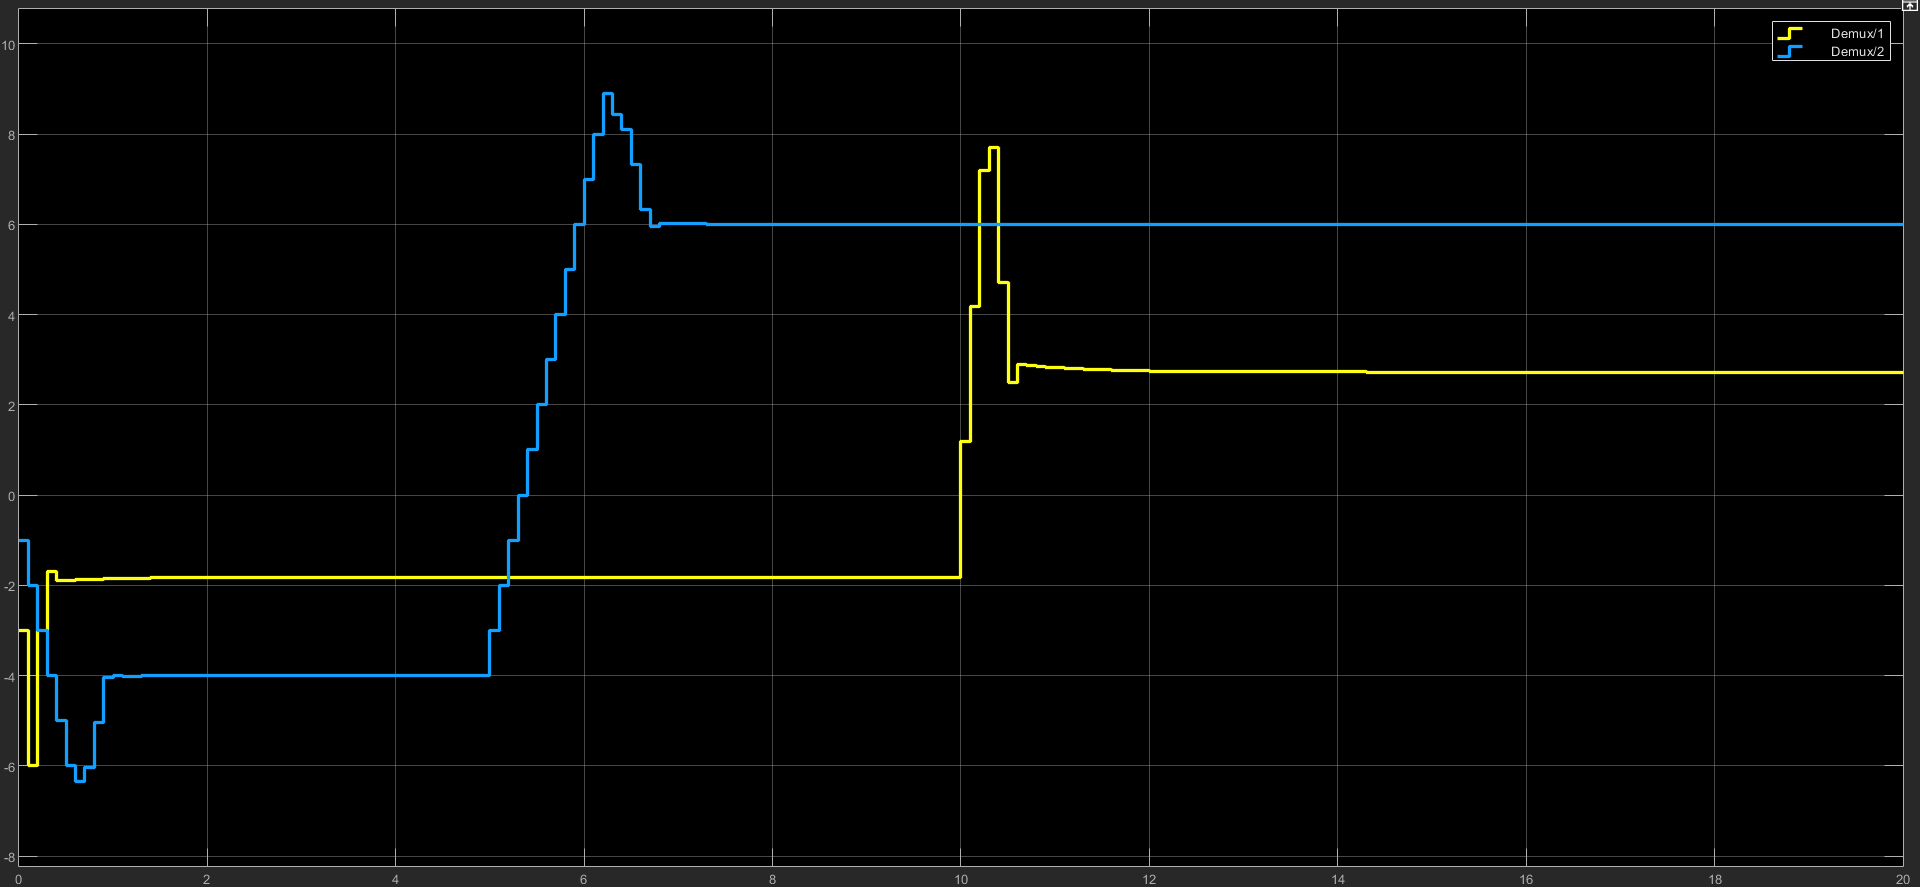
\includegraphics[scale = 0.3]{Q2_sim_control_consmall.png}
	\caption{خروجی کنترلر با
		نرخ تغییر با بازه کوچکتر}
\end{figure}

با کاهش بازه نرخ تغییرات، سیستم کند شده که این امر دور از انتظار هم نیست چراکه کنترلر مجبور است با فاصله زمانی بیشتر و درنتیجه در بازه طولانی‌تری سیگنال مورد نیاز سیستم را تولید کند.
\newpage
حال برای نرخ تغییر با بازه بزرگتر خروجی‌ها را بررسی می‌کنیم.\\
\[
-8 W/min \leq \dot{u}_1 \leq 8 W/min
\]
\[
-5 W/min \leq \dot{u}_2 \leq 5 W/min
\]
\begin{figure}[h!]
	\centering
	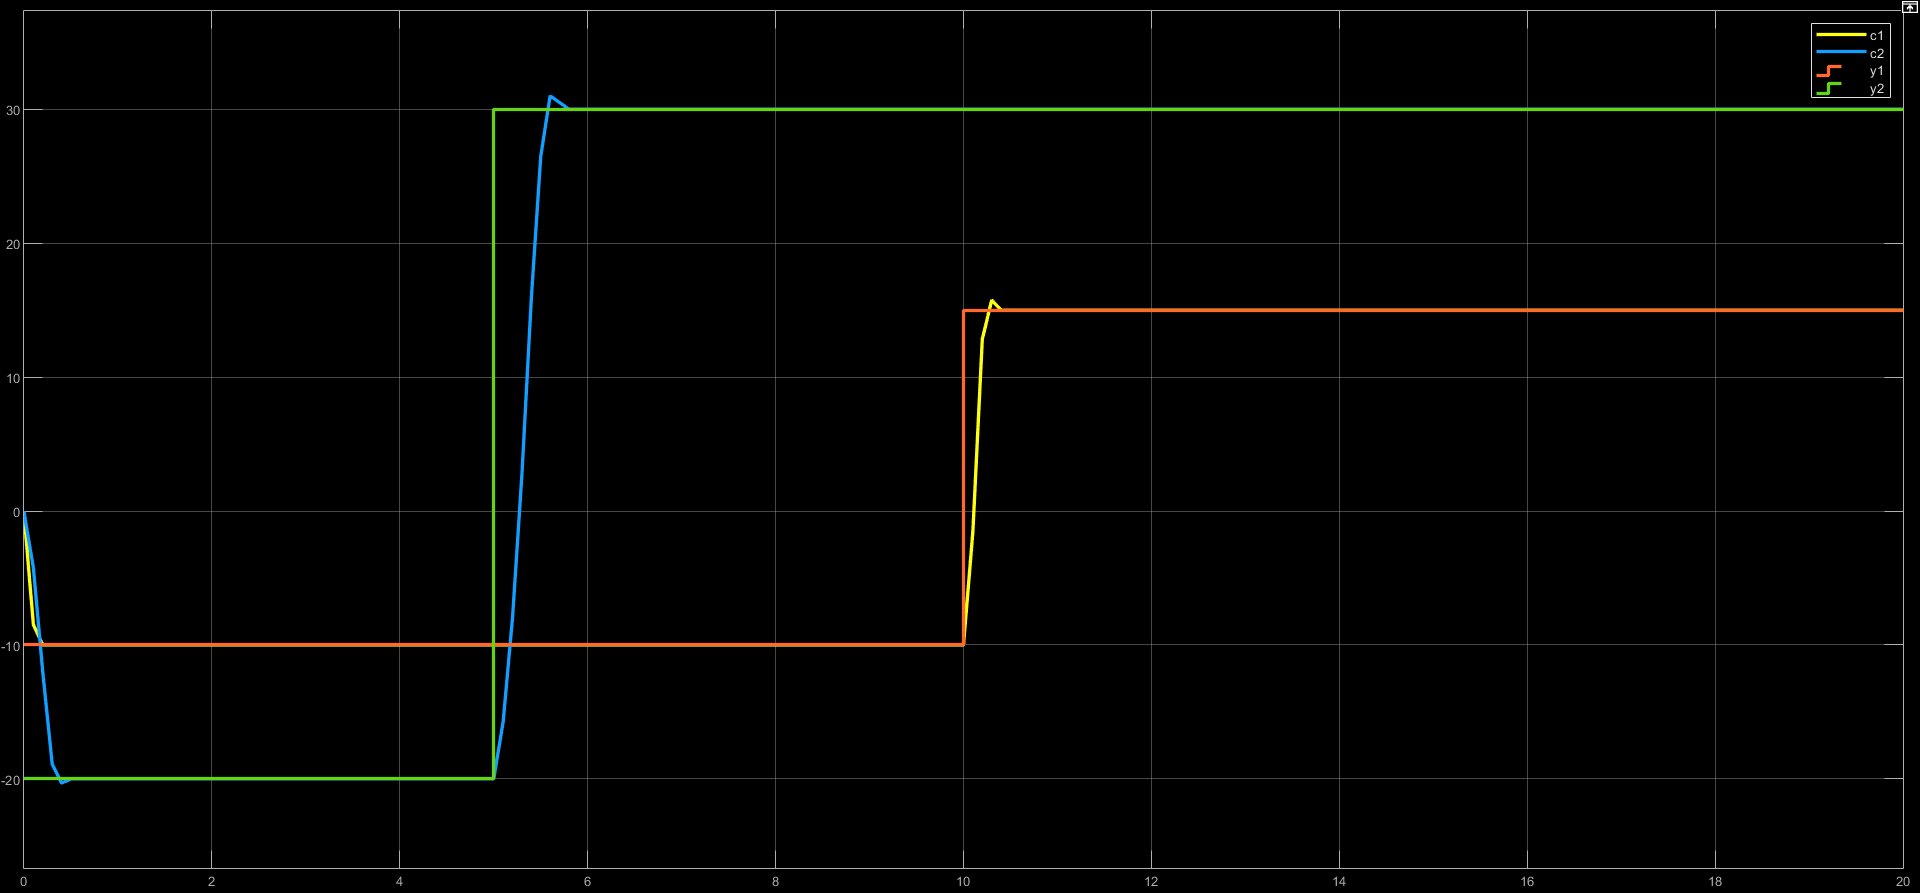
\includegraphics[scale = 0.3]{Q2_sim_result_conbig.png}
	\caption{خروجی سیستم کنترل شده با
		نرخ تغییر با بازه بزرگتر}
\end{figure}
\begin{figure}[h!]
	\centering
	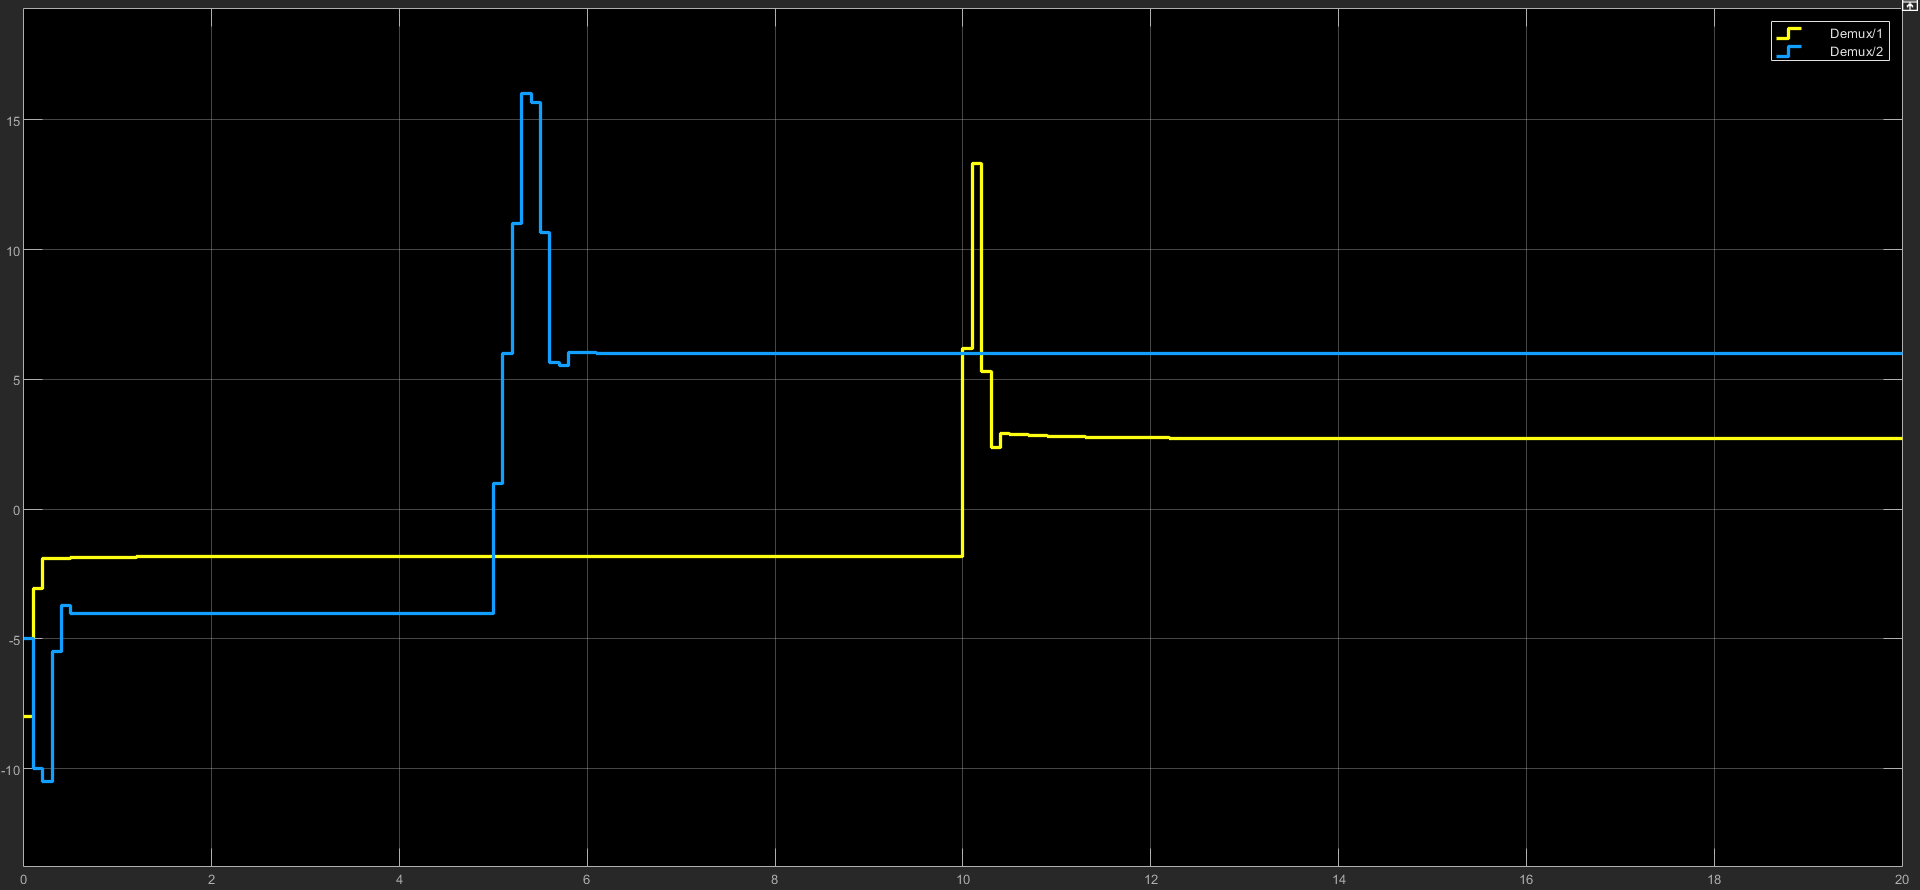
\includegraphics[scale = 0.3]{Q2_sim_control_conbig.png}
	\caption{خروجی کنترلر با
		نرخ تغییر با بازه بزرگتر}
\end{figure}

با افزایش بازه نرخ تغییرات، سیستم سریعتر شده که این امر نیز دور از انتظار نیست چراکه کنترلر مجبور است با فاصله زمانی کمتری و درنتیجه در بازه کوتاه‌تری سیگنال مورد نیاز سیستم را تولید کند.

\newpage
\subsubsection{\lr{Weights}}
برای بررسی اثر وزن‌ها، یکبار مقدار یکسان و یکبار برعکس قسمت قبل درنظر می‌گیریم و مقایسه می‌کنیم.\\
ابتدا حالت یکسان بودن وزن‌ها را بررسی می‌کنیم.\\
\[
R = \begin{bmatrix}
	0.1 & 0 \\
	0 & 0.1
\end{bmatrix}
\]
\[
Q = \begin{bmatrix}
	15 & 0 \\
	0 & 15
\end{bmatrix}
\]
\begin{figure}[h!]
	\centering
	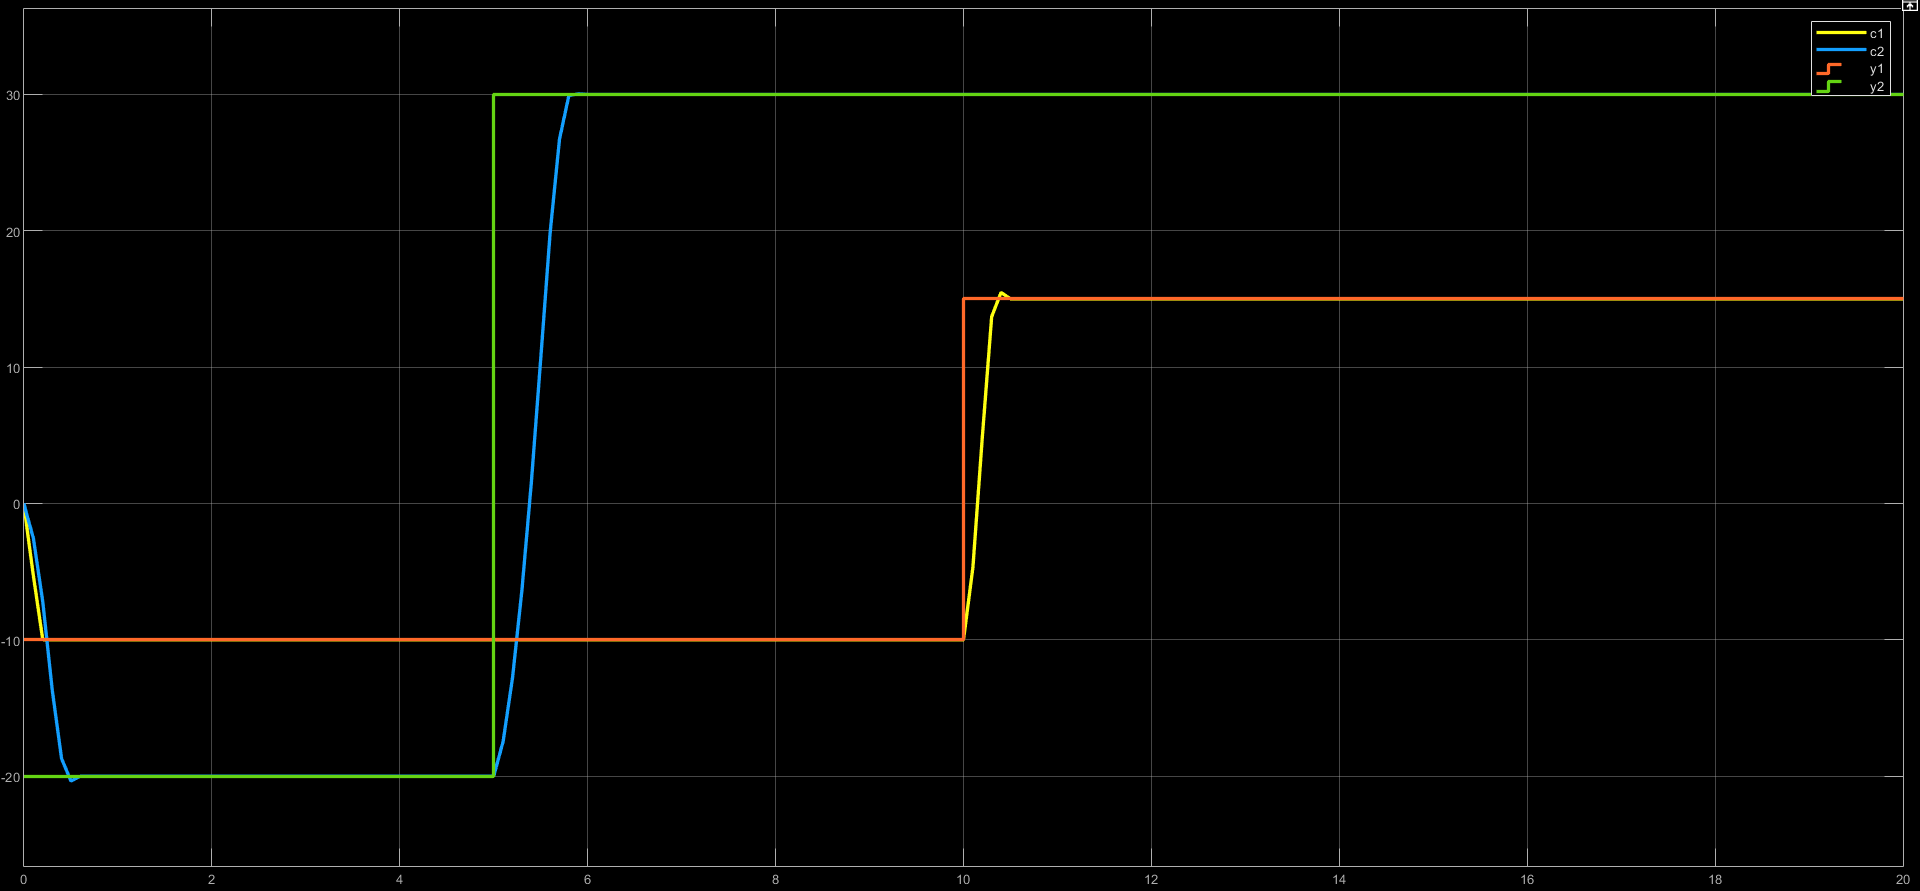
\includegraphics[scale = 0.3]{Q2_sim_result_weightsame.png}
	\caption{خروجی سیستم کنترل شده با
		وزن‌های یکسان}
\end{figure}
\begin{figure}[h!]
	\centering
	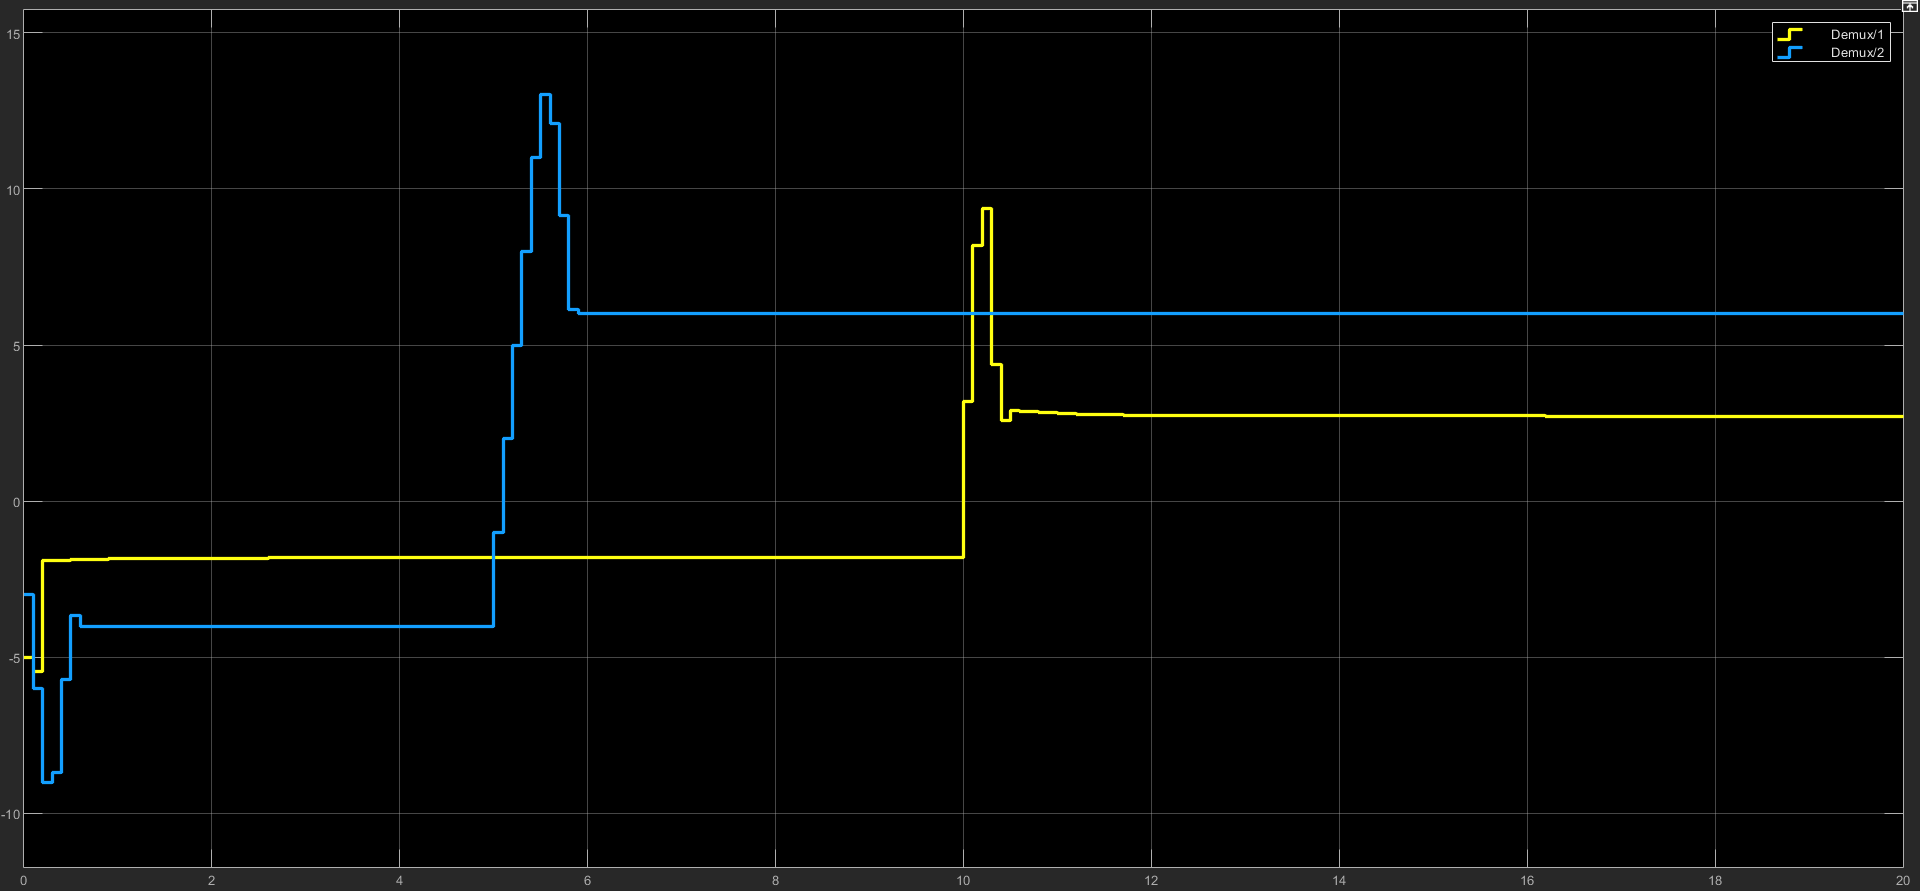
\includegraphics[scale = 0.3]{Q2_sim_control_weightsame.png}
	\caption{خروجی کنترلر با
		وزن‌های یکسان}
\end{figure}

با توجه به سایر پارامترهای مسئله، تغییر محسوسی در جواب‌ها مشخص نیست ولی با توجه به کارکرد ماتریس وزن‌ها، با کوچک کردن
\lr{R}
کنترلر تلاش می‌کند تا با تغییزات بیشتر در ورودی، خطای خروجی را با سرعت بیشتری کاهش دهد.\\
و برای ماتریس 
\lr{Q}
با قراردادن مقادیر متفاوت برای خروجی‌ها، کنترلر سعی می‌کند تا خروجی با وزن بالاتر را سریعتر کنترل کند.
\newpage
حال برای وزن‌ها اعداد متفاوت درنظر می‌گیریم و اولویت‌ها را برعکس سوال قرار می‌دهیم.\\
\[
R = \begin{bmatrix}
	0.2 & 0 \\
	0 & 0.1
\end{bmatrix}
\]
\[
Q = \begin{bmatrix}
	25 & 0 \\
	0 & 15
\end{bmatrix}
\]

با اعمال این تغییرات، بازهم تغییر قابل مشاهده‌ای رخ نداد اما همان توضیحاتی که در قسمت قبل بیان شد، گویای نتایج هست.
\newpage
\section{سوال سوم}


























\end{document} 
